\chapter{Energy Efficiency of DBMS}
\label{cha:Results}


This chapter presents the benchmarks obtained when running the four DBMS considered in this master thesis . The systems are executed via the HammerDB framework, and the RAPL and Arduino energy monitoring systems are used to collect their energy consumption while running in the same hardware and software conditions.
%\discuss{Talvez considerar j+a duas secções/paragrafos: single user e depois multiple user}
\section{Benchmark Results}

In this section we will present and analyse in great detail the performance of the MySQL, MariaDB, Postgres, and Redis DBMS.  We consider the energy consumed for each DBMS when executed by HammerDB both in a single user mode, and when multiple users are performing DBMS actions. Moreover, we distinguish the energy consumed by the Packgage, estimated by RAPL, and the energy consumed by the hard disk, as measure by the Arduino system. Concerning the RAPL estimations, we will consider the estimation provided by RAPL package metric: it includes the consumption of the Packgage cores, DRAM and other components of the chip.  

As described in Chapter~\ref{cha:middle} HammerDB computes two DBMS specific performance metrics: the transactions per minute and the new orders per minute. Obviously, different DBMS may show different \textit{per minute} performances, which can have an impact on energy consumption. Thus, we will analyse  the impact of such HammerDB metrics on both Packgage and disk energy consumption. 



\subsection{DBMS in Single User: Energy Consumption}


%Figure~\ref{fig:bocplotyenergy} includes the box plot of the energy consumption of each \gls{dbms}.  For the HammerDB metrics, similar graphs are presented in Figures~\ref{fig:medianhammerdb}.
%and \ref{fig:bocplothammer}. The box plot representation uses the median, the approximate quartiles, and the lowest and highest data points to convey the level, spread, and symmetry of a distribution of data values. It can also be easily refined to identify outlier data values and can be easily constructed by hand~\cite{doi:10.7326/0003-4819-110-11-916}.  

%As finals graphs of single user are the  energy consumption per HammerDB Metrics. We see in Figure \ref{fig:mediantpmenergy} the energy consumption per \gls{tpm} and Figure \ref{fig:mediannopmenergy} the  energy consumption per \gls{nopm} for all subsystems.  Similar to how we presented the energy consumption and HammerDB results and metrics, Figure  \ref{fig:bocplottrans} shows a box plot for the energy consumption per \gls{tpm} and in Figure \ref{fig:bocplotnumber} the box plot for the energy consumption per \gls{nopm}. In both cases, they also display the package, disk, and global amount.


    First will discuss energy consumption on every level for every DBMS with only one virtual user. Figure \ref{fig:medianenergy} shows the median values, and Figure \ref{fig:bocplotyenergy} shows the distribution of these values in a box plot. Here we can see the median, the approximate quartiles, the lowest and highest data points to convey the level, spread, and symmetry of a distribution of data values~\cite{doi:10.7326/0003-4819-110-11-916}.

\begin{figure}[H]
\centering
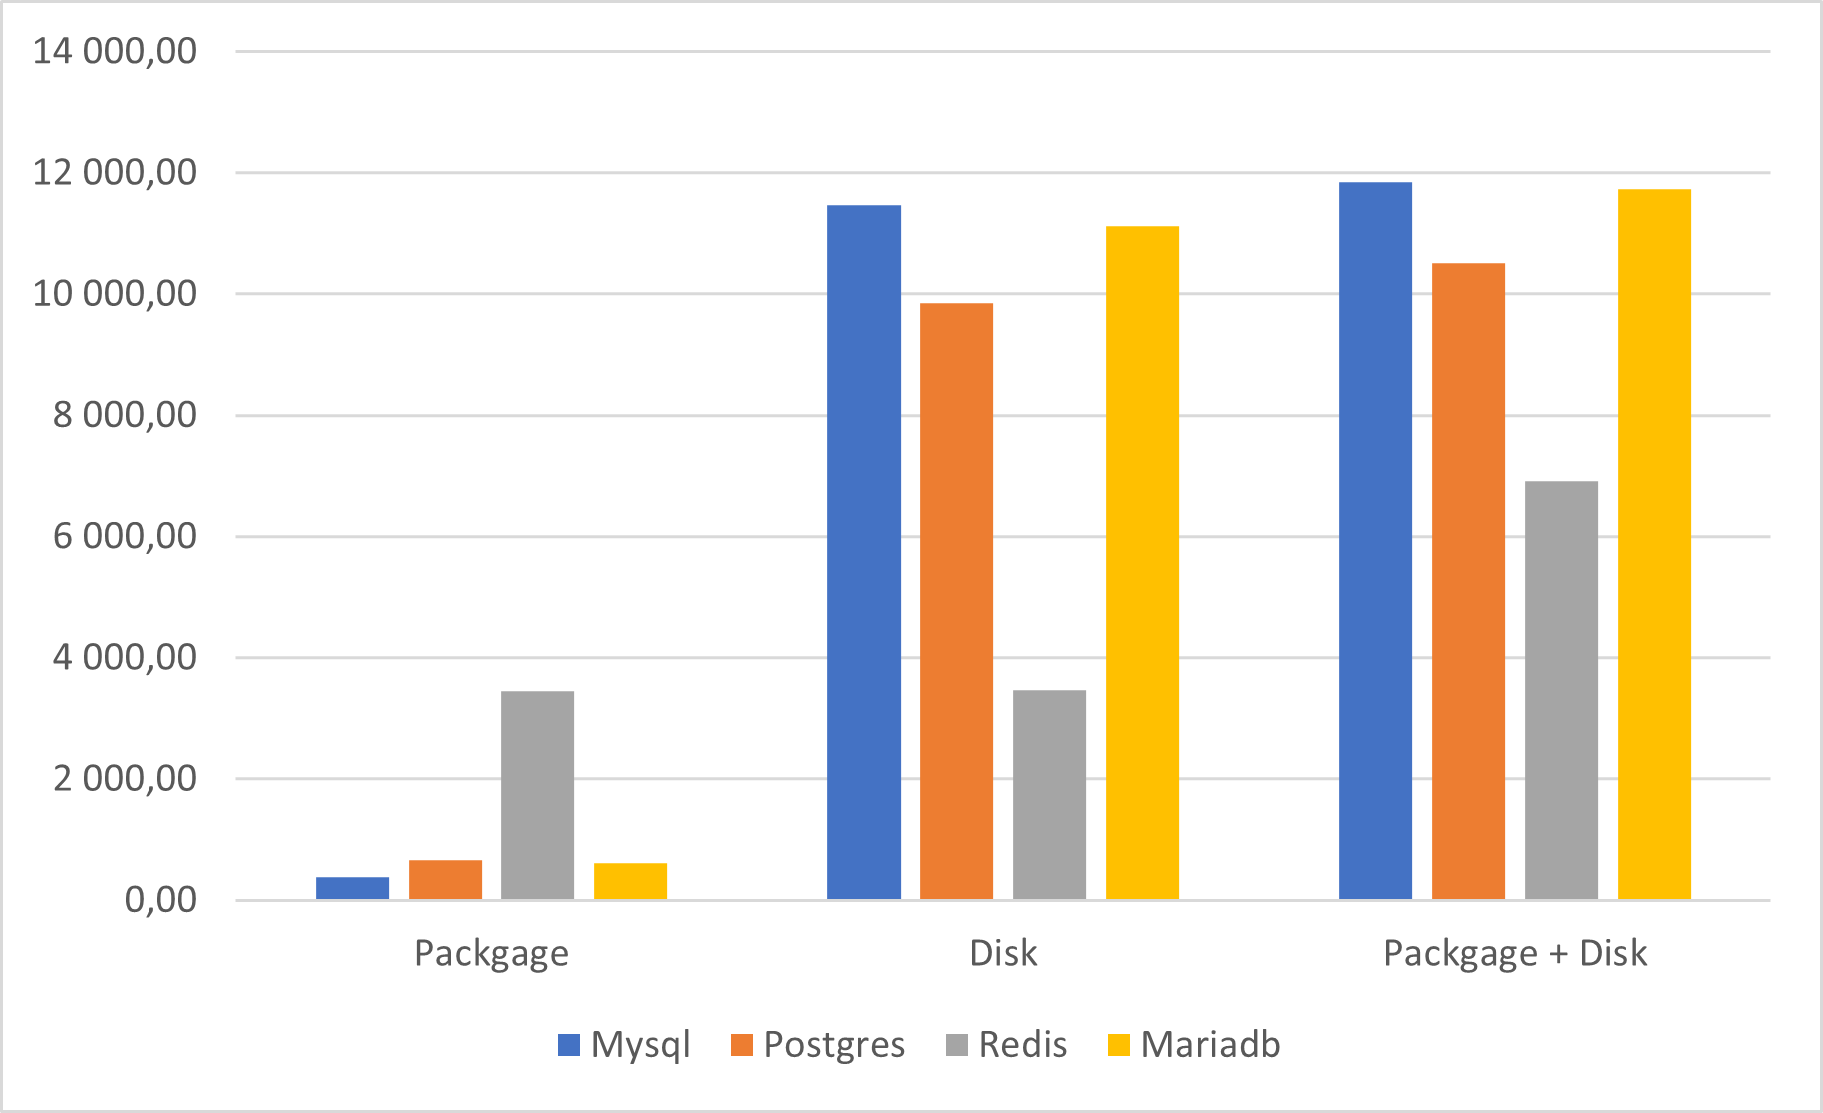
\includegraphics[width=0.8\columnwidth]{results/median/energy.png}
\caption{Median of energy consumption on Package, Disk and Total.}
\label{fig:medianenergy}
\end{figure}

     Looking at the package measurements, Redis shows the highest consumption energy median value, followed by  Postgres, MariaDB, and MySQL. We can see that all relational DBMS have a lower energy consumption compared to Redis.
	
    The inverse of the Package level happens at the disk level, where the relational DBMS spends in median the most energy and the non-relational spends the least. In this situation, MySQL was the one that spent the most afterward was MariaDB and then Postgres and lastly Redis.

    It is important to notice even though Redis spent in median more than the others on the Package level, the energy he saves on the disk pays off in terms of total energy consumption, making it the least expensive one, followed by MariaDB, Postgres, and MySQL. The reason for this is that secondary storage has a higher effect than the Package on the overall energy consumed.

%Explicação destes possiveis Valores de energy:

    The measured values can be explained by Redis being a non-relational DBMS of type Key-Value where the data is stored in-memory explains why the consumption on disk is low comparing with the Relational DBMS. This naturally implies a higher consumption on the Package level since use of cache affect energy consumption on the Package \cite{10.55552505464}.
    
%REF redis in action

%Exposiçao da sua distribuição
%Figure Here we can see the median, the approximate quartiles, the lowest and highest data points to convey the level, spread, and symmetry of a distribution of data values~\cite{doi:10.7326/0003-4819-110-11-916}.
\newpage
   \begin{figure*}[h]
        \centering
        \begin{subfigure}[b]{0.325\textwidth}
            \centering
			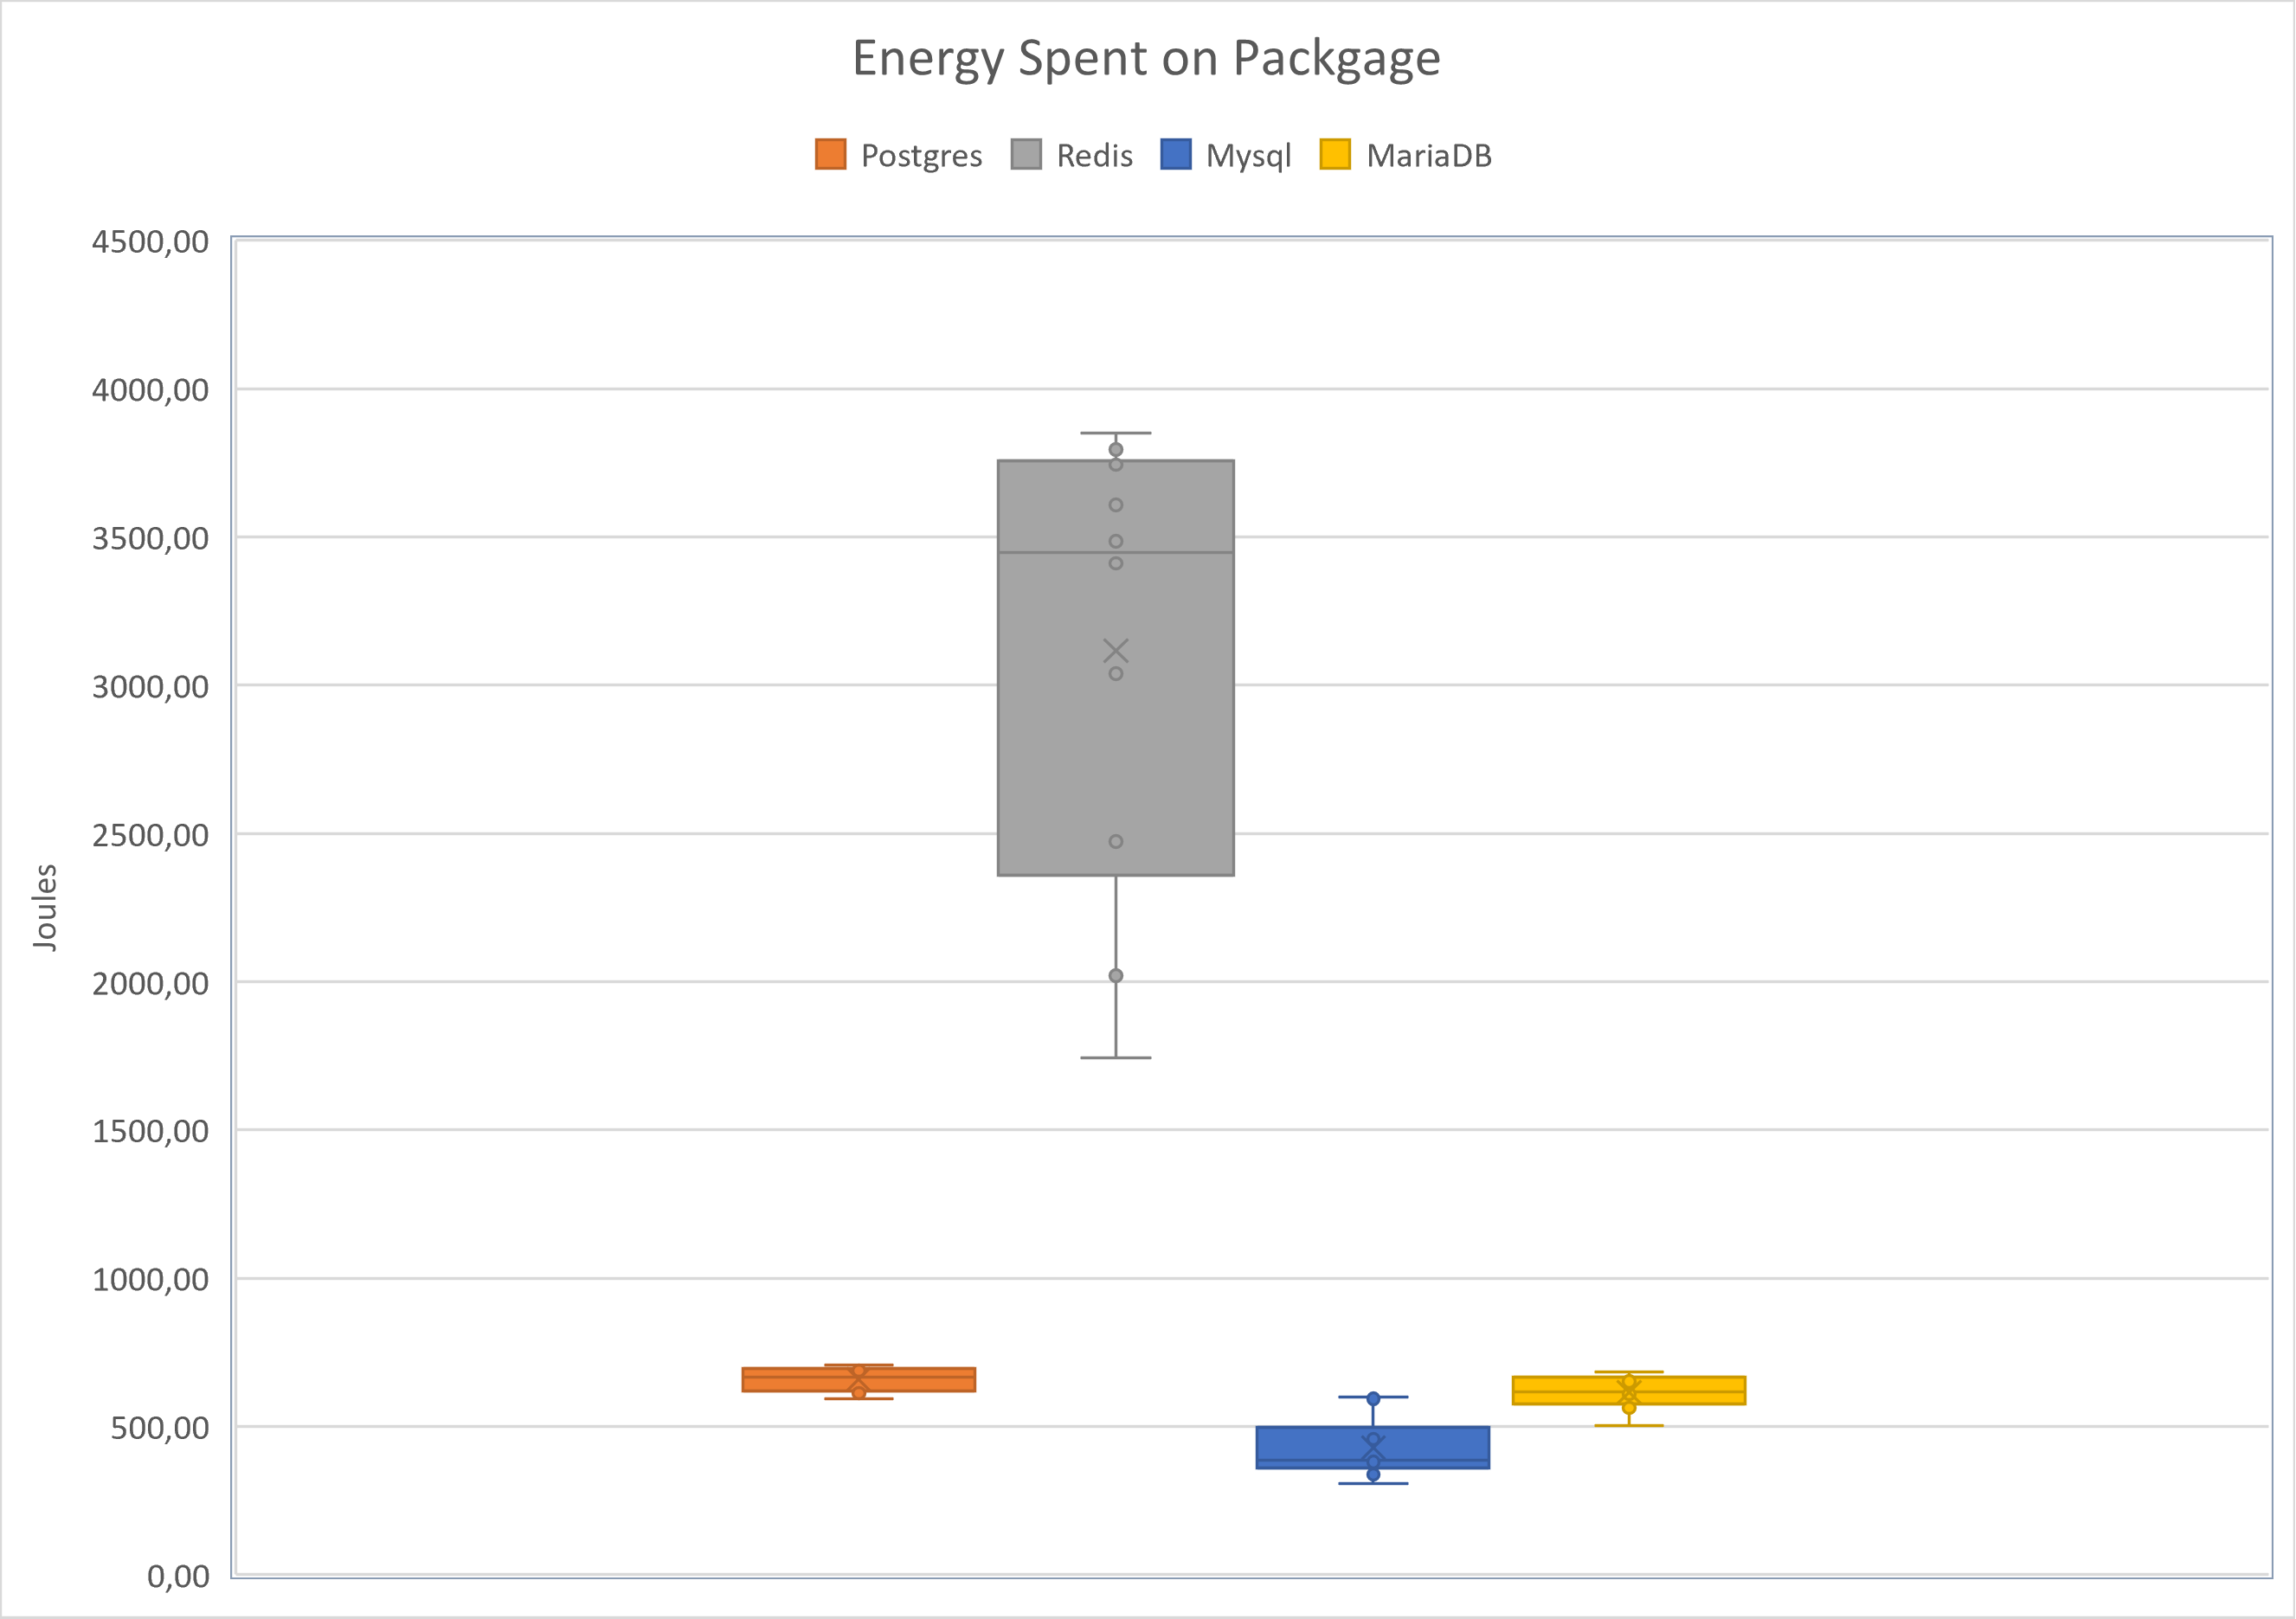
\includegraphics[width=1\columnwidth]{results/boxplot/Packgage.png}
			\caption[Distribution of energy consumed on Package]%
            {{\small Distribution of energy consumed on Package}}    
			\label{fig:bocplotyenergyPackage}
        \end{subfigure}
        \begin{subfigure}[b]{0.325\textwidth}   
            \centering 
            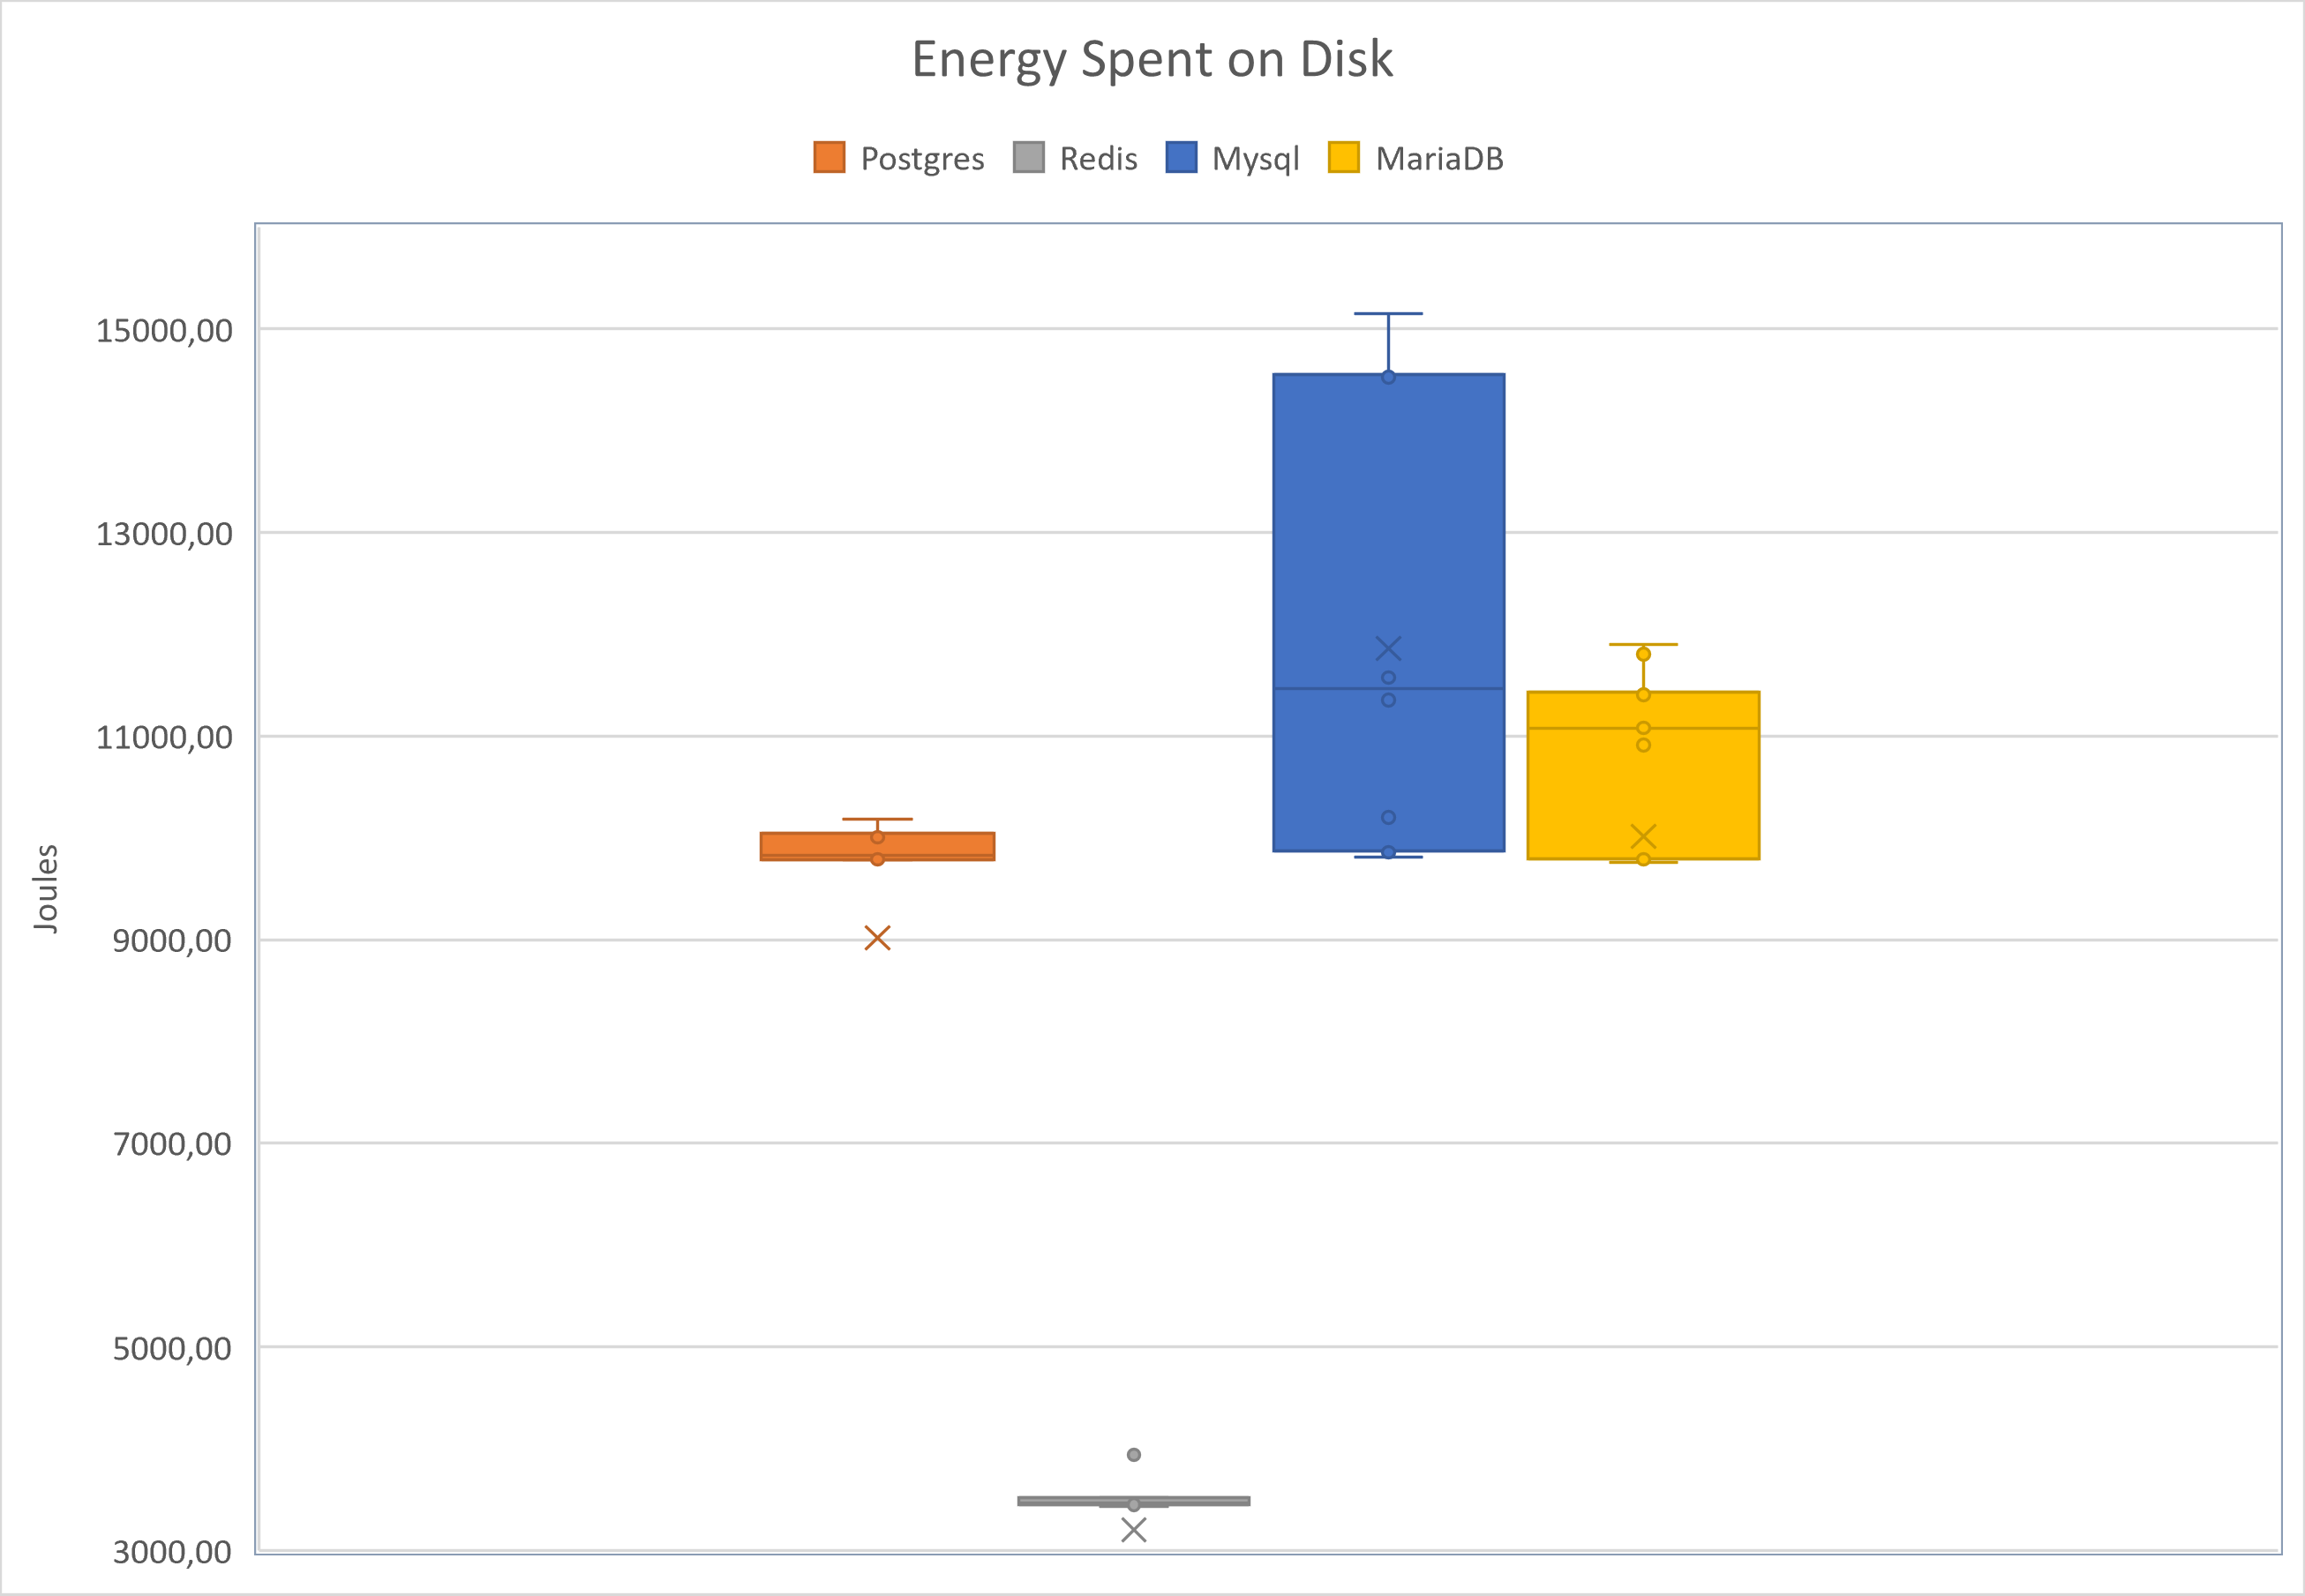
\includegraphics[width=1\columnwidth]{results/boxplot/Disk.png}
            \caption[Distribution of energy consumed on Disk]%
            {{\small Distribution of energy consumed on Disk}}    
            \label{fig:bocplotyenergydisk}
        \end{subfigure}
        \begin{subfigure}[b]{0.325\textwidth}   
            \centering 
			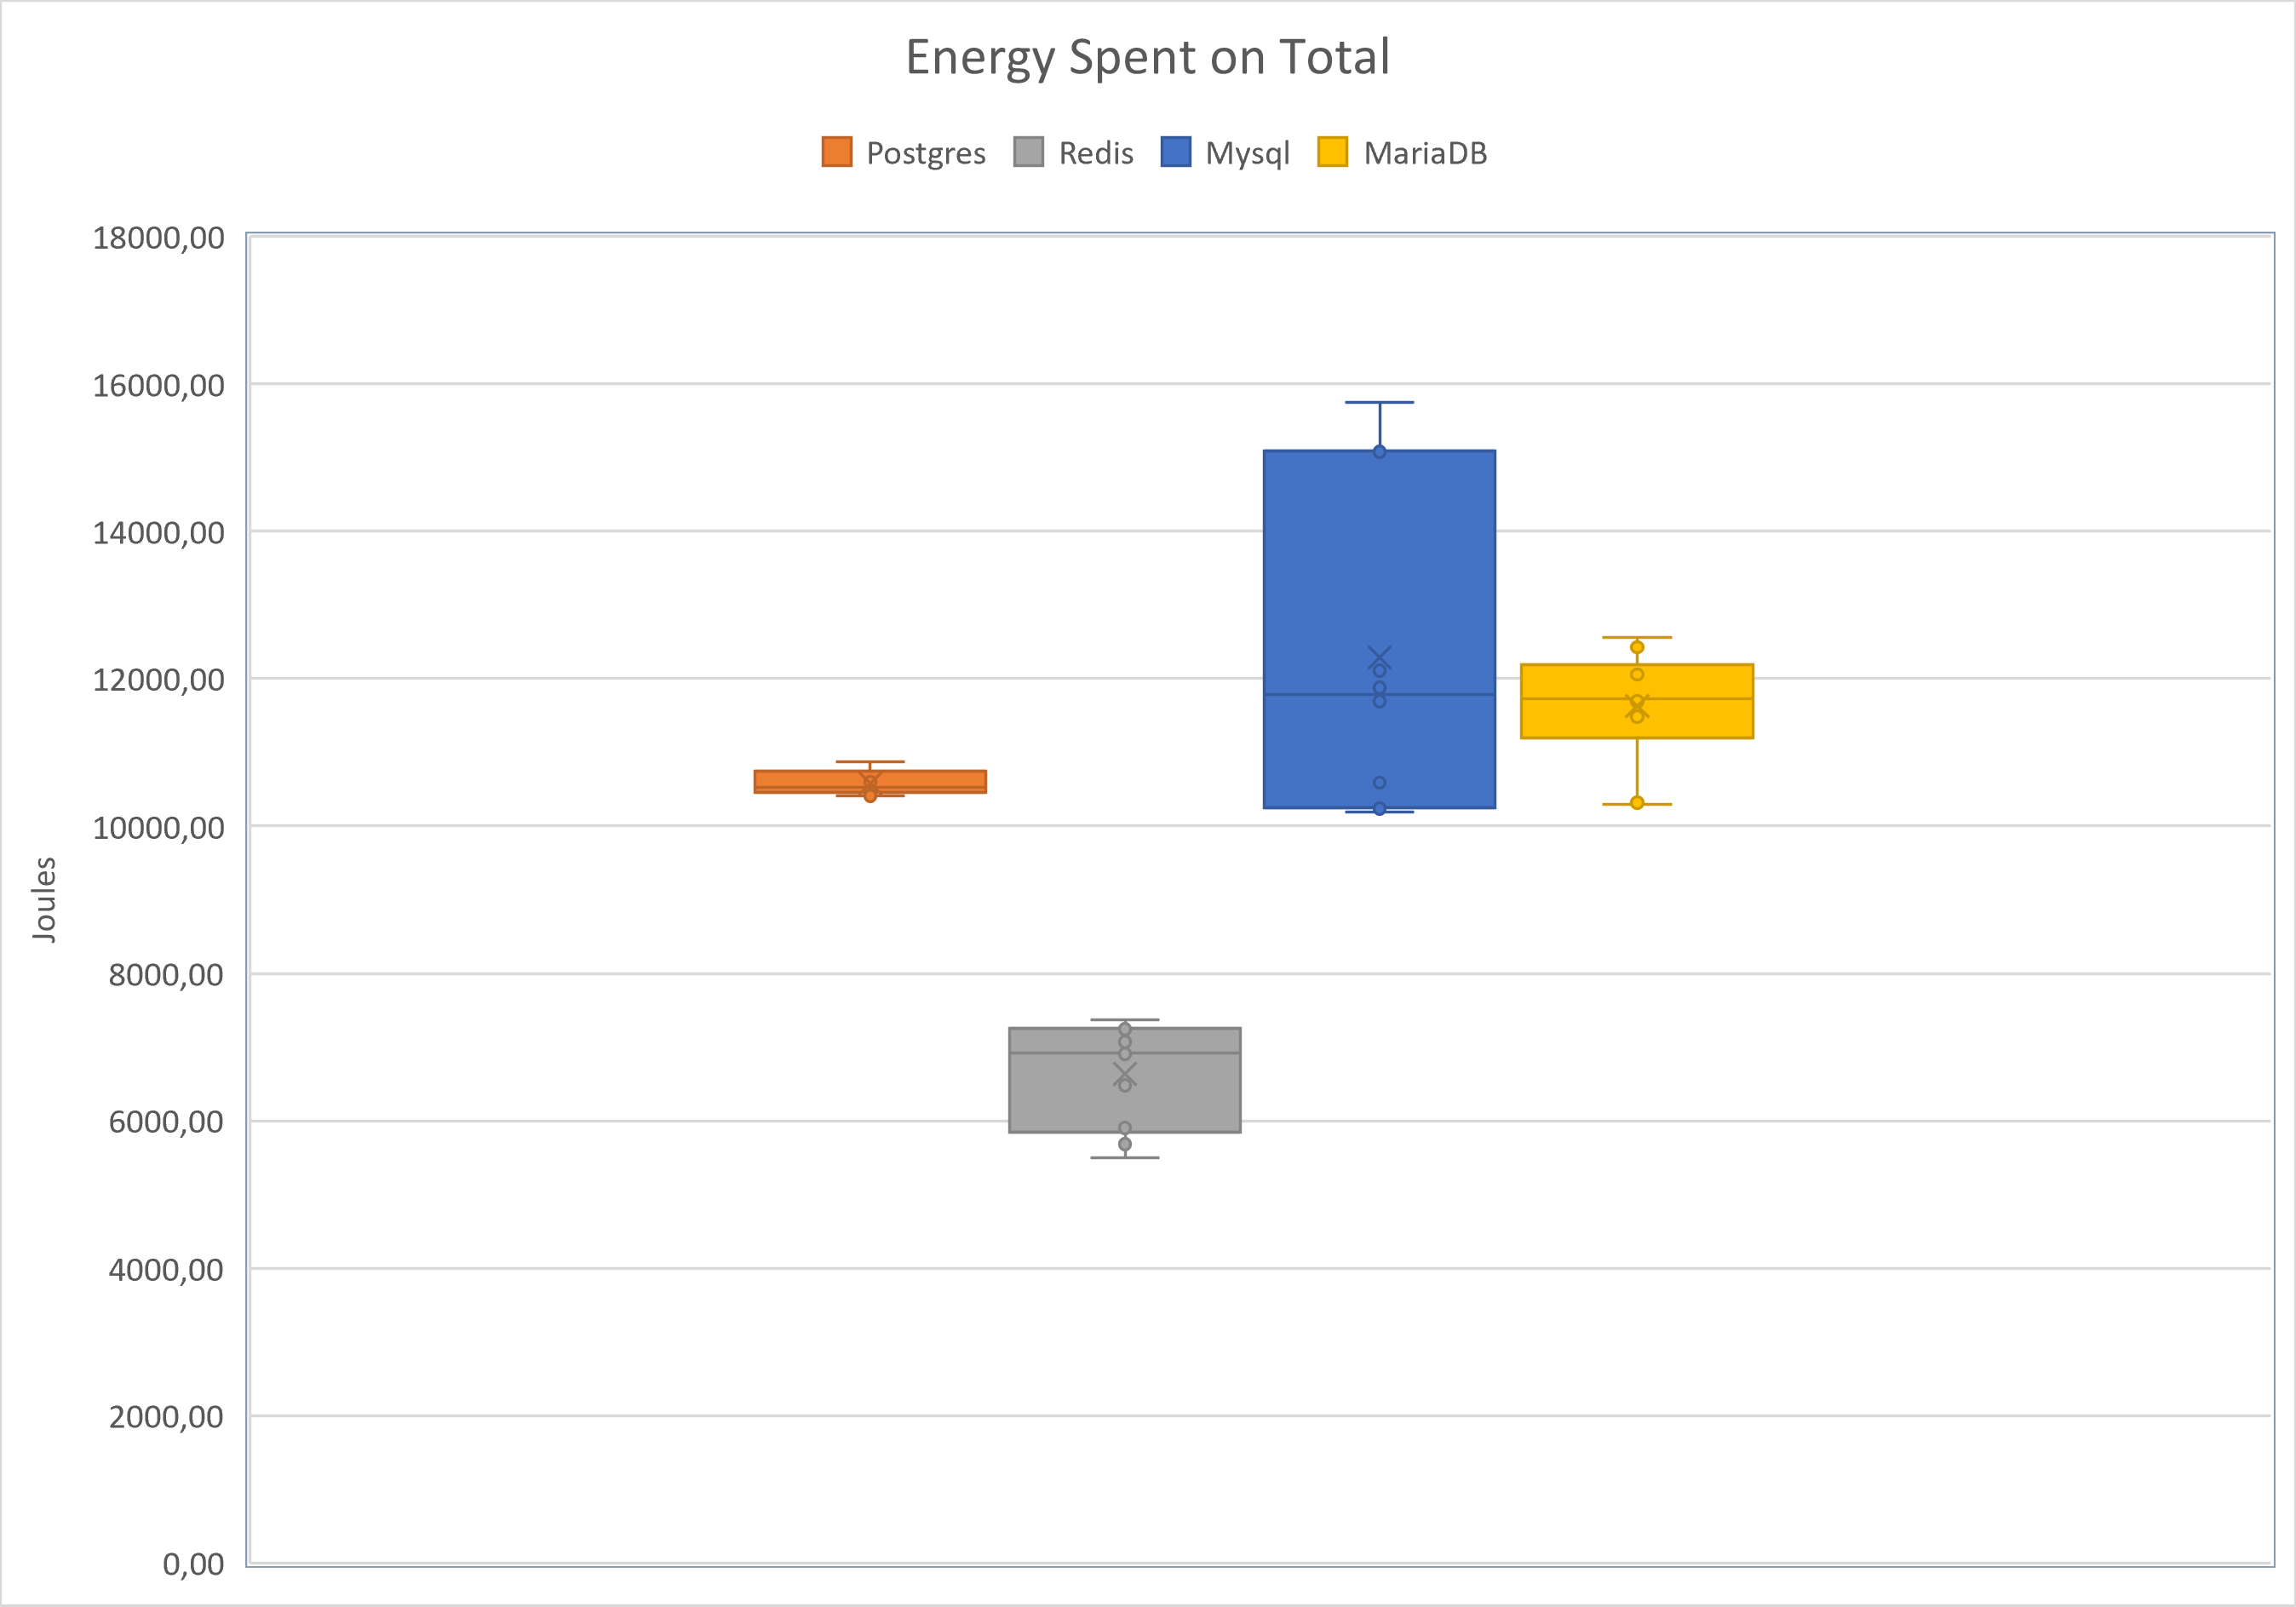
\includegraphics[width=1\columnwidth]{results/boxplot/Total.png}
            \caption[Distribution of energy consumed on Overall System]%
            {{\small Distribution of energy consumed on Overall System}}    
            \label{fig:bocplotyenergytotal}
        \end{subfigure}
        \caption[ Distribution of energy consumed ]
        {\small Distribution of energy consumed} 
        \label{fig:bocplotyenergy}
    \end{figure*}

	
	When talking about the distribution of the values between the different executions, we can see in Figure \ref{fig:bocplotyenergyPackage} that the distribution on the Package level is smaller on the relational databases, and Redis has a large magnitude distribution on values of energy consumption.
    Also, it is worth mentioning a specific case in relational DBMS. Although, on average, Postgres is the most expensive of relational DBMS, the maximum energy consumption made by MySQL and MariaDB surpass the minimum energy consumption of Postgres.
	
	In secondary storage, seen in Figure \ref{fig:bocplotyenergydisk}, there is almost no variation of  Redis results, and the same case occurs in Postgres, but the distribution in MySQL and MariaDB is wide. The median between MySQL and MariaDB was very close. But when observing both distributions on this level, we can see the magnitude of the values of MySQL is a lot bigger comparing with MariaDB. Here also worth mention that the maximum of Postgres surpasses the minimum of both MySQL and MariaDB.


%Frase complicada
    As it happens with the median of energy consumption, the distribution of total energy consumed follows almost the same pattern of distribution of energy consumed of the disk because of the impact it has on total energy consumed where the distribution of MySQL remains the most significant. These values are presented in Figure  \ref{fig:bocplotyenergytotal}.
    

%%Performance 

\paragraph{Runtime Performance}
Now discussing the HammerDB metrics, similar graphs are presented in Figures~\ref{fig:medianhammerdb} for the median of these metrics and Figure \ref{fig:bocplothammer} for the distribution.

As seen in Figure \ref{fig:medianhammerdb}, Redis has a much better performance, in terms of TPM, than any relational DBMS. We can also see a relationship between TPM with less consumption in the disk.
When talking about NOPM, Postgres is the one with better performance.
MariaDB and Redis have the same number of NOPM, and the lowest is MySQL. Here the results are very close, and there's not much margin between them, and here can't be draw any conclusion between energy consumption and performance.



\begin{figure}[H]
\centering
    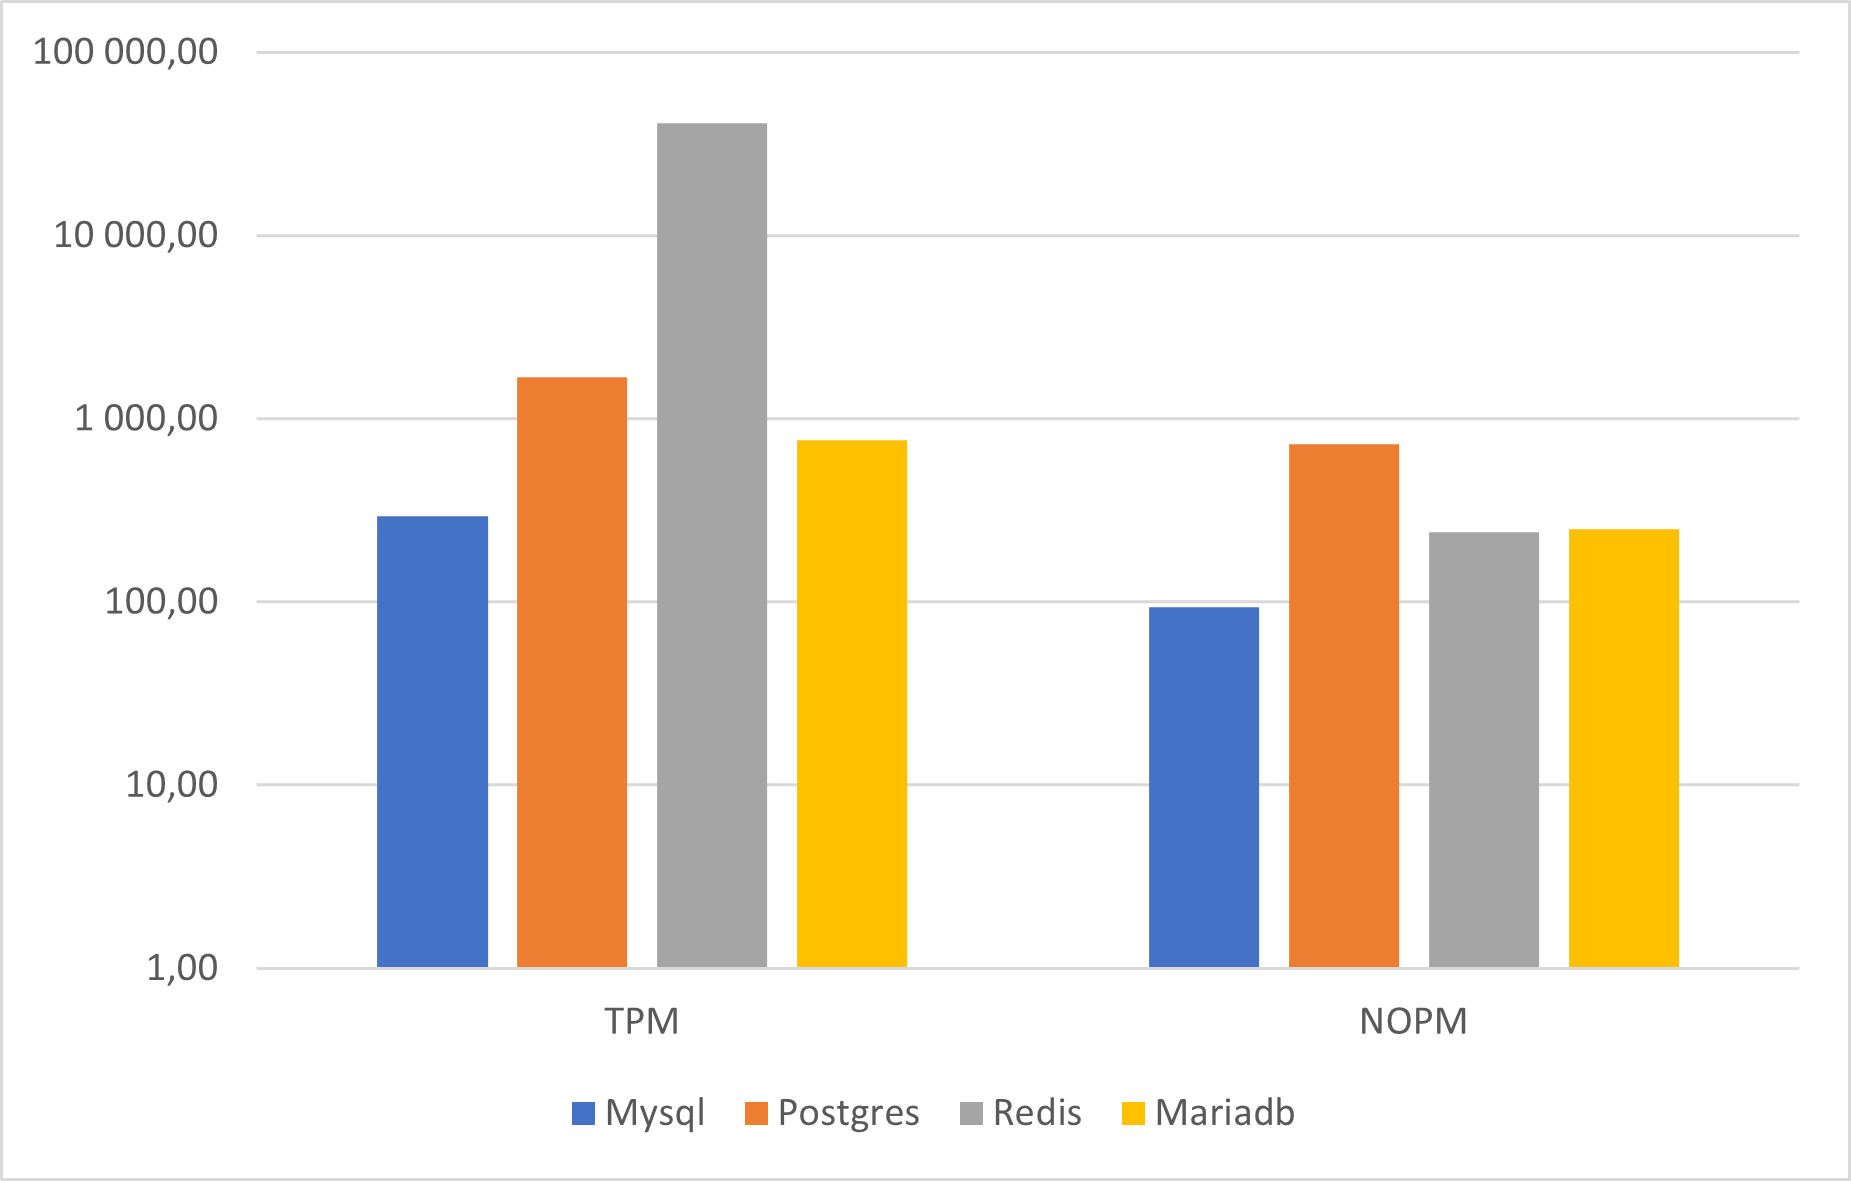
\includegraphics[width=0.8\columnwidth]{results/median/hammerdb.png}
\caption{Median of HammerDB results.}
\label{fig:medianhammerdb}
\end{figure}


When look at the HammerDB results, \gls{tpm} distribution between different tests doesn't have much variation except on Redis where the variation is noted  in Figure \ref{fig:bocplothammerTPM}. 
When looking at the distribution of \gls{nopm} in Figure \ref{fig:bocplothammerNOPM}, we can see that it doesn't have much variation between different DBMS the only thing worth mention is that even knowing that MariaDB and Redis have the same median, Redis has a larger distribution meaning that in some executions Redis can have worst performance than MariaDB.

   \begin{figure*}[!ht]
        \centering
        \begin{subfigure}[b]{0.32\textwidth}
            \centering
			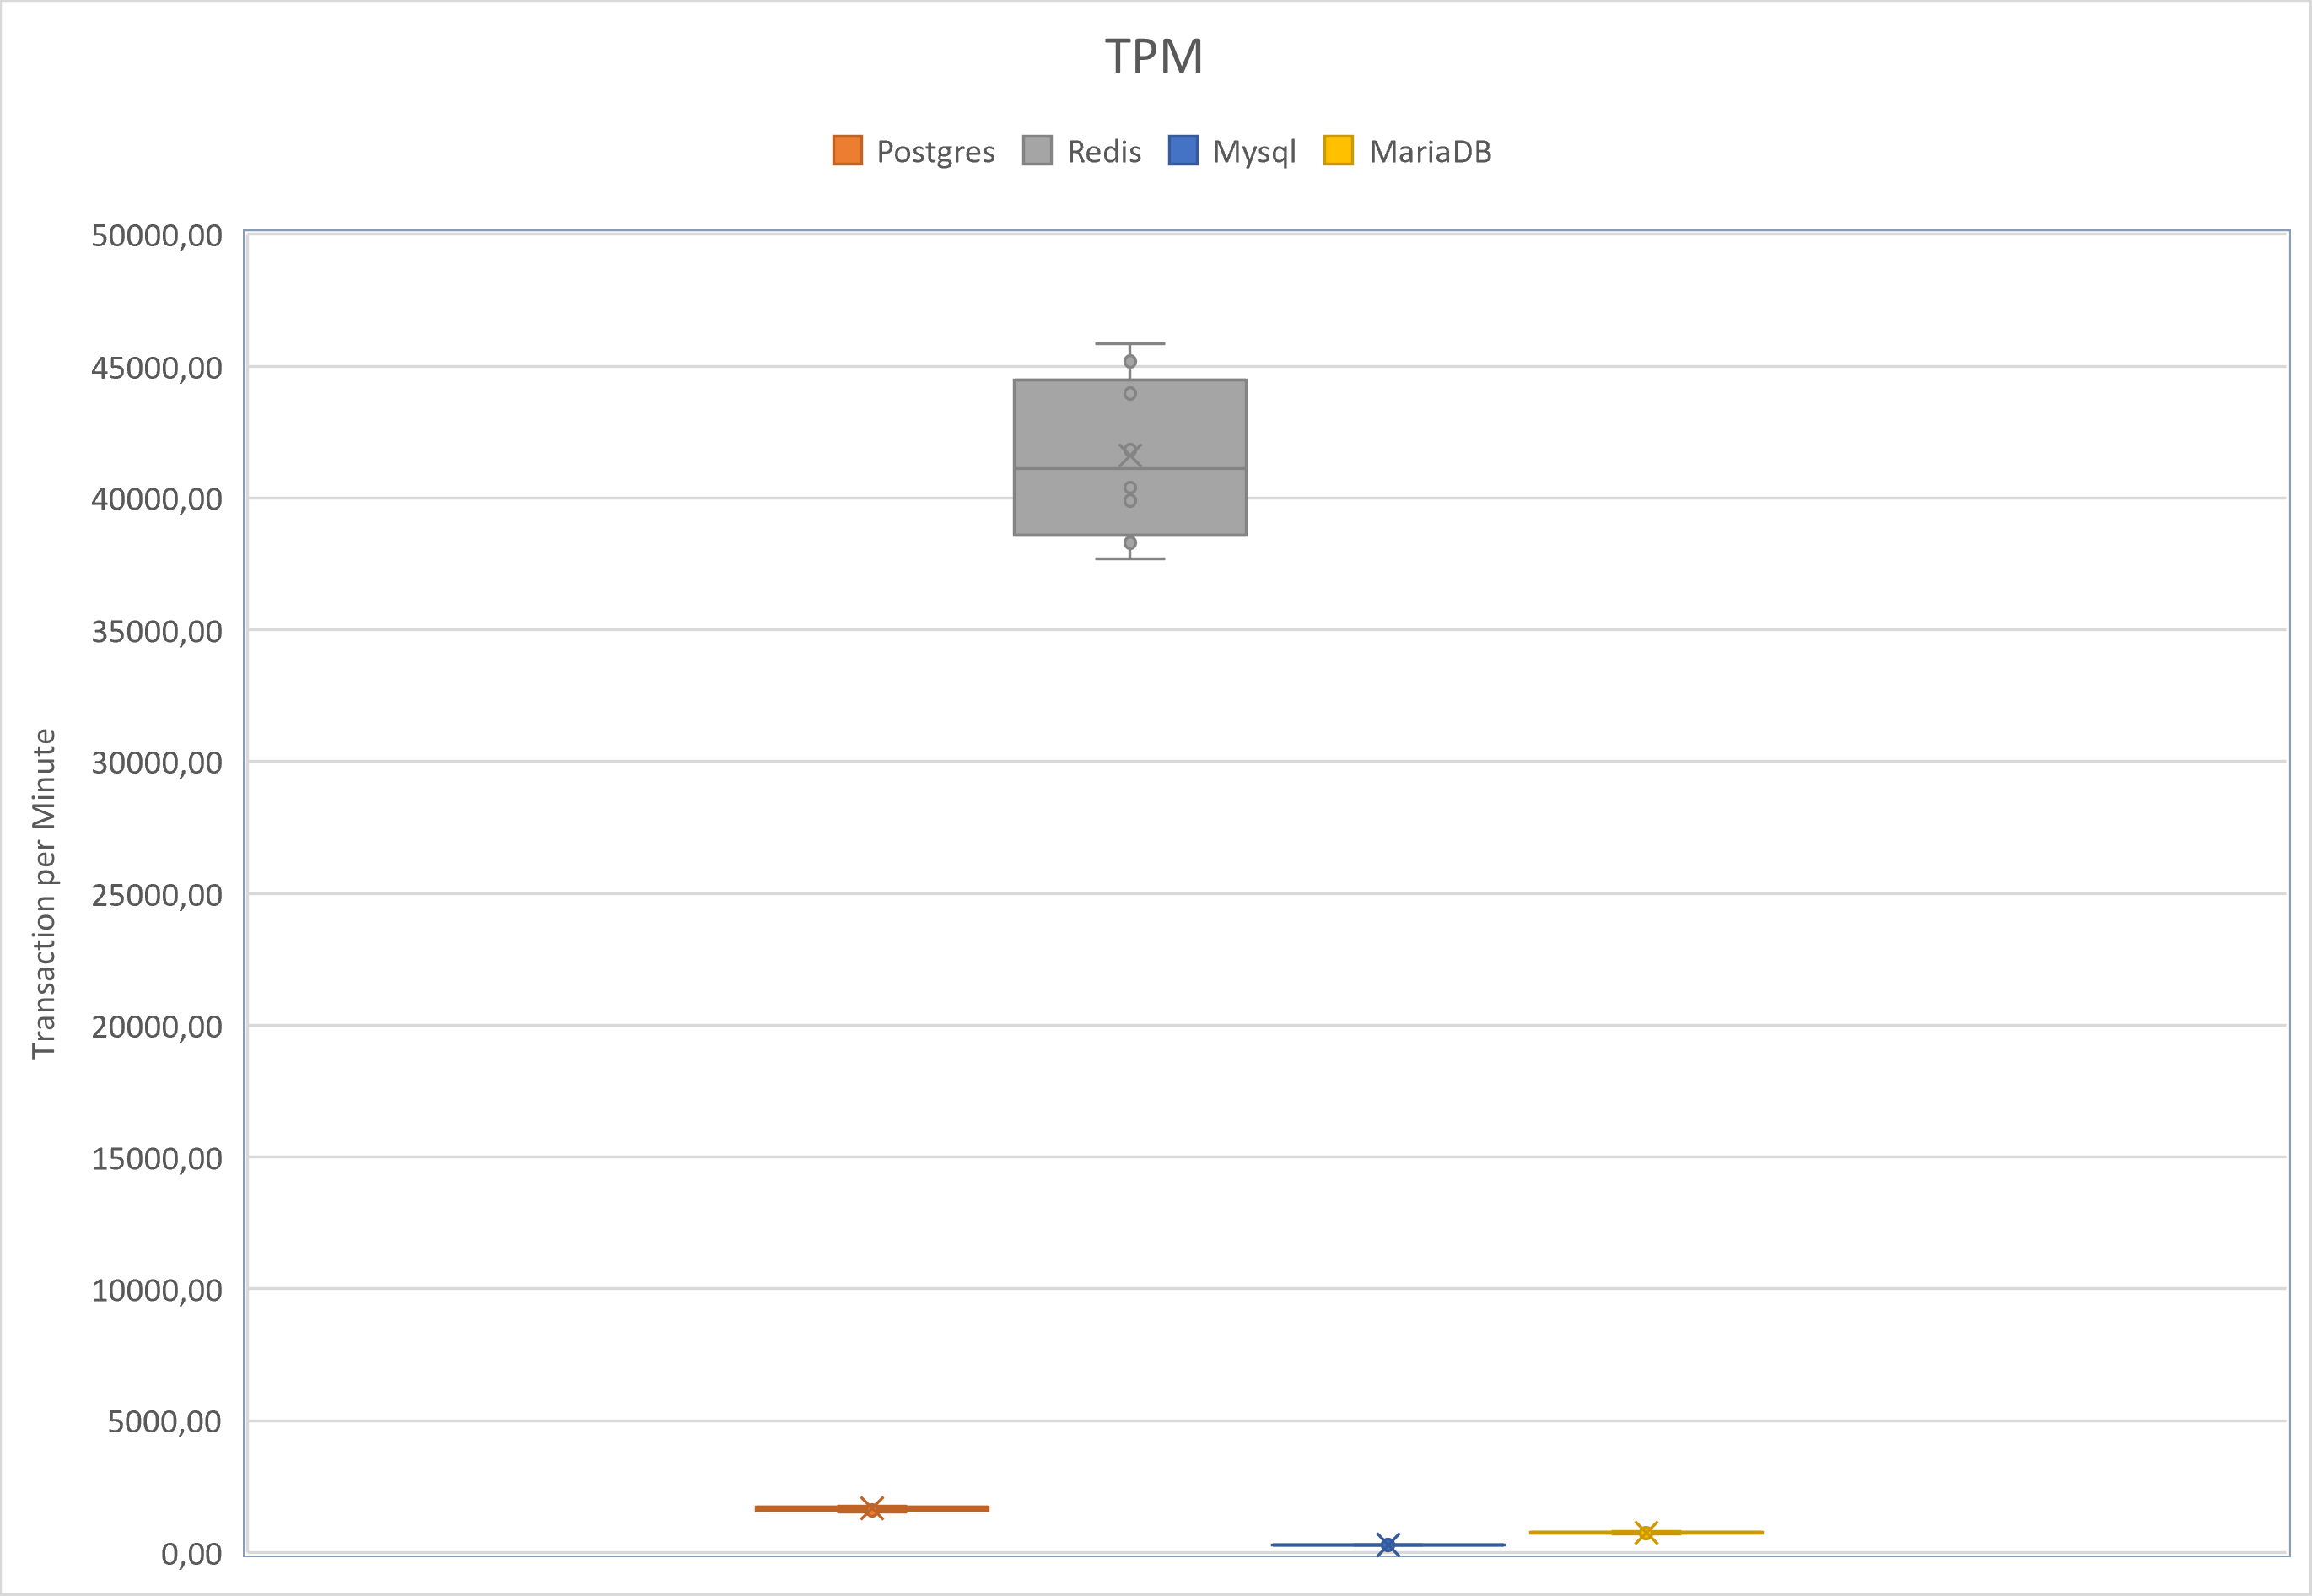
\includegraphics[width=1\columnwidth]{results/boxplot/TPM.png}
			\caption[]%
            {{\small Distribution of TPM}}    
			\label{fig:bocplothammerTPM}
        \end{subfigure}
        \begin{subfigure}[b]{0.32\textwidth}  
            \centering 
            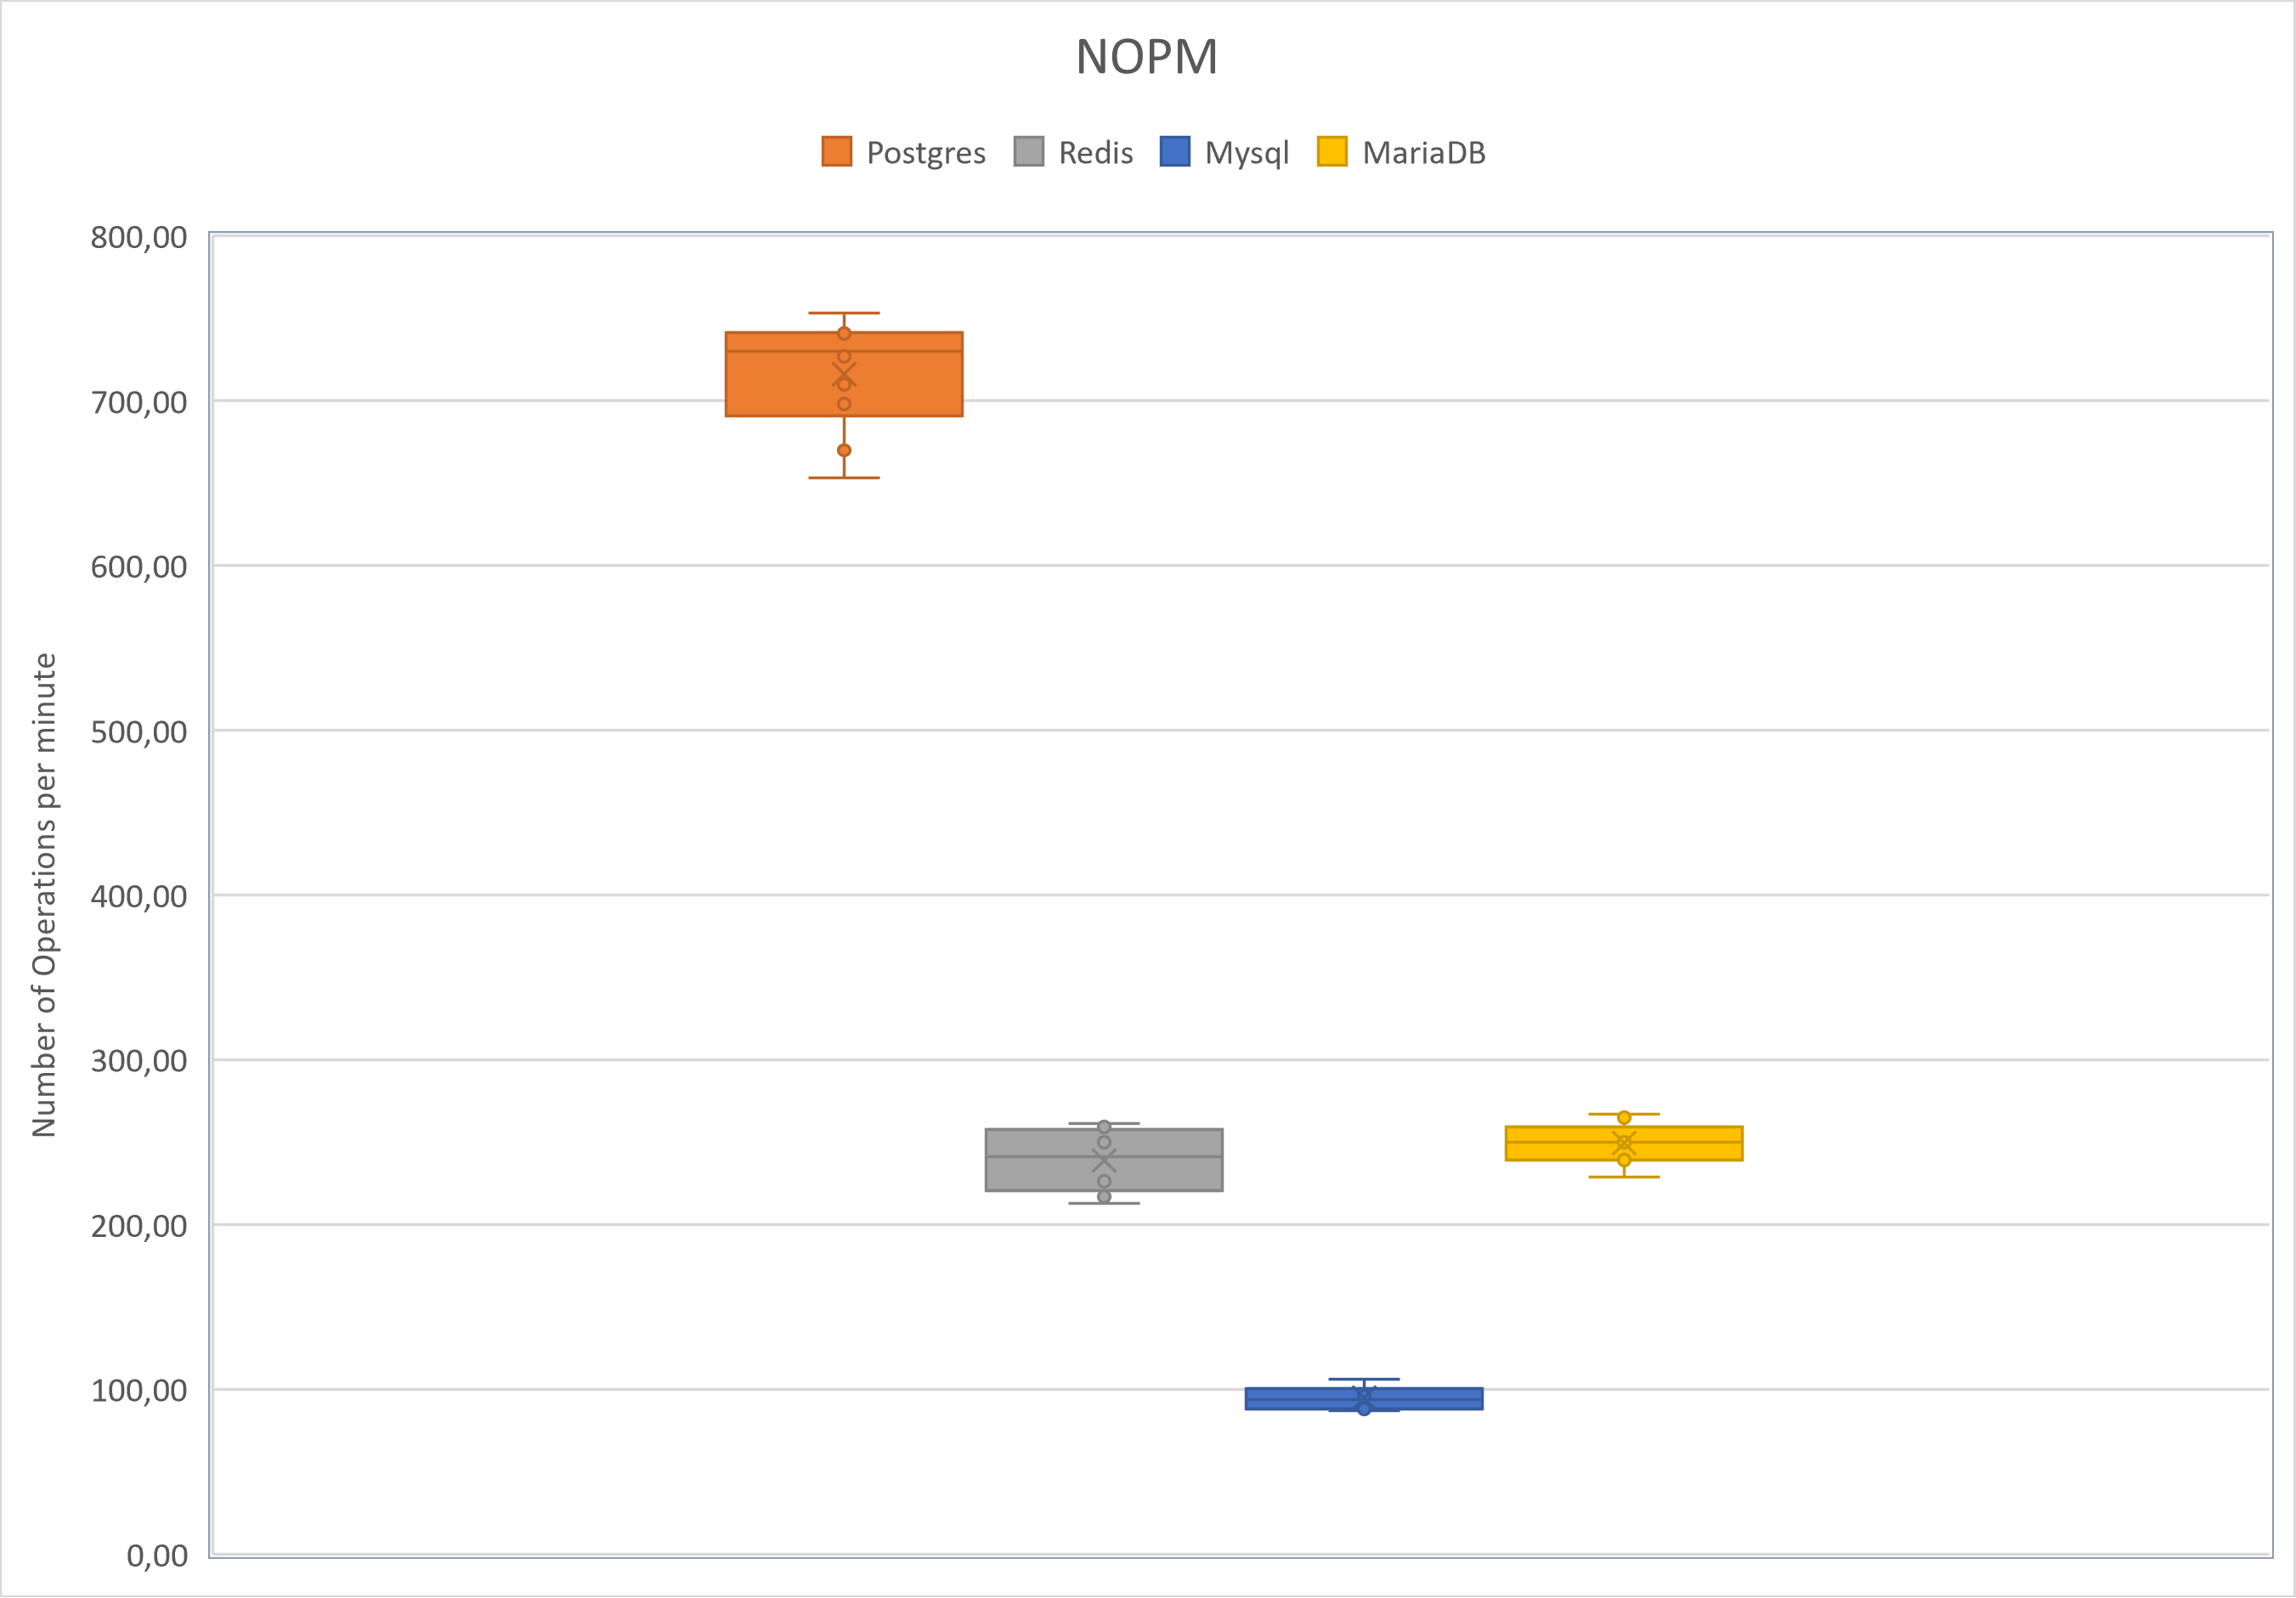
\includegraphics[width=1\columnwidth]{results/boxplot/NOPM.png}
            \caption[]%
            {{\small Distribution of NOPM}}    
            \label{fig:bocplothammerNOPM}
        \end{subfigure}
        \vskip\baselineskip
        \caption[ Distribution of performance on HammerDB results]
        {\small Distribution of HammerDB results} 
        \label{fig:bocplothammer}
    \end{figure*}
   



\paragraph{Energy Consumption per Runtime Performance} 

The last discussion of singer users is the Energy Consumption per HammerDB metrics. For Energy Consumption per TPM, Figure \ref{fig:mediantpmenergy} for the median of Energy Consumption Per TPM and Figure \ref{fig:bocplottrans} for the distribution of Energy Consumption Per TPM. For the Energy Consumption per NOPM, Figures \ref{fig:mediannopmenergy} for the median of Energy Consumption Per NOPM and Figure \ref{fig:bocplotnumber} for the distribution of Energy Consumption Per NOPM.




In terms of Joules per \gls{tpm} on the package, disk, and total, as seen in Figure \ref{fig:mediantpmenergy}, it follows the same trend of the most expensive in terms of energy consumption where the MySQL is the most expensive followed by MariaDB, Postgres, and Redis. The distribution of these values in Figure \ref{fig:bocplottrans} show that MySQL is always the most expensive followed by MariaDB, Postgres, and Redis.

\begin{figure}[H]
\centering
    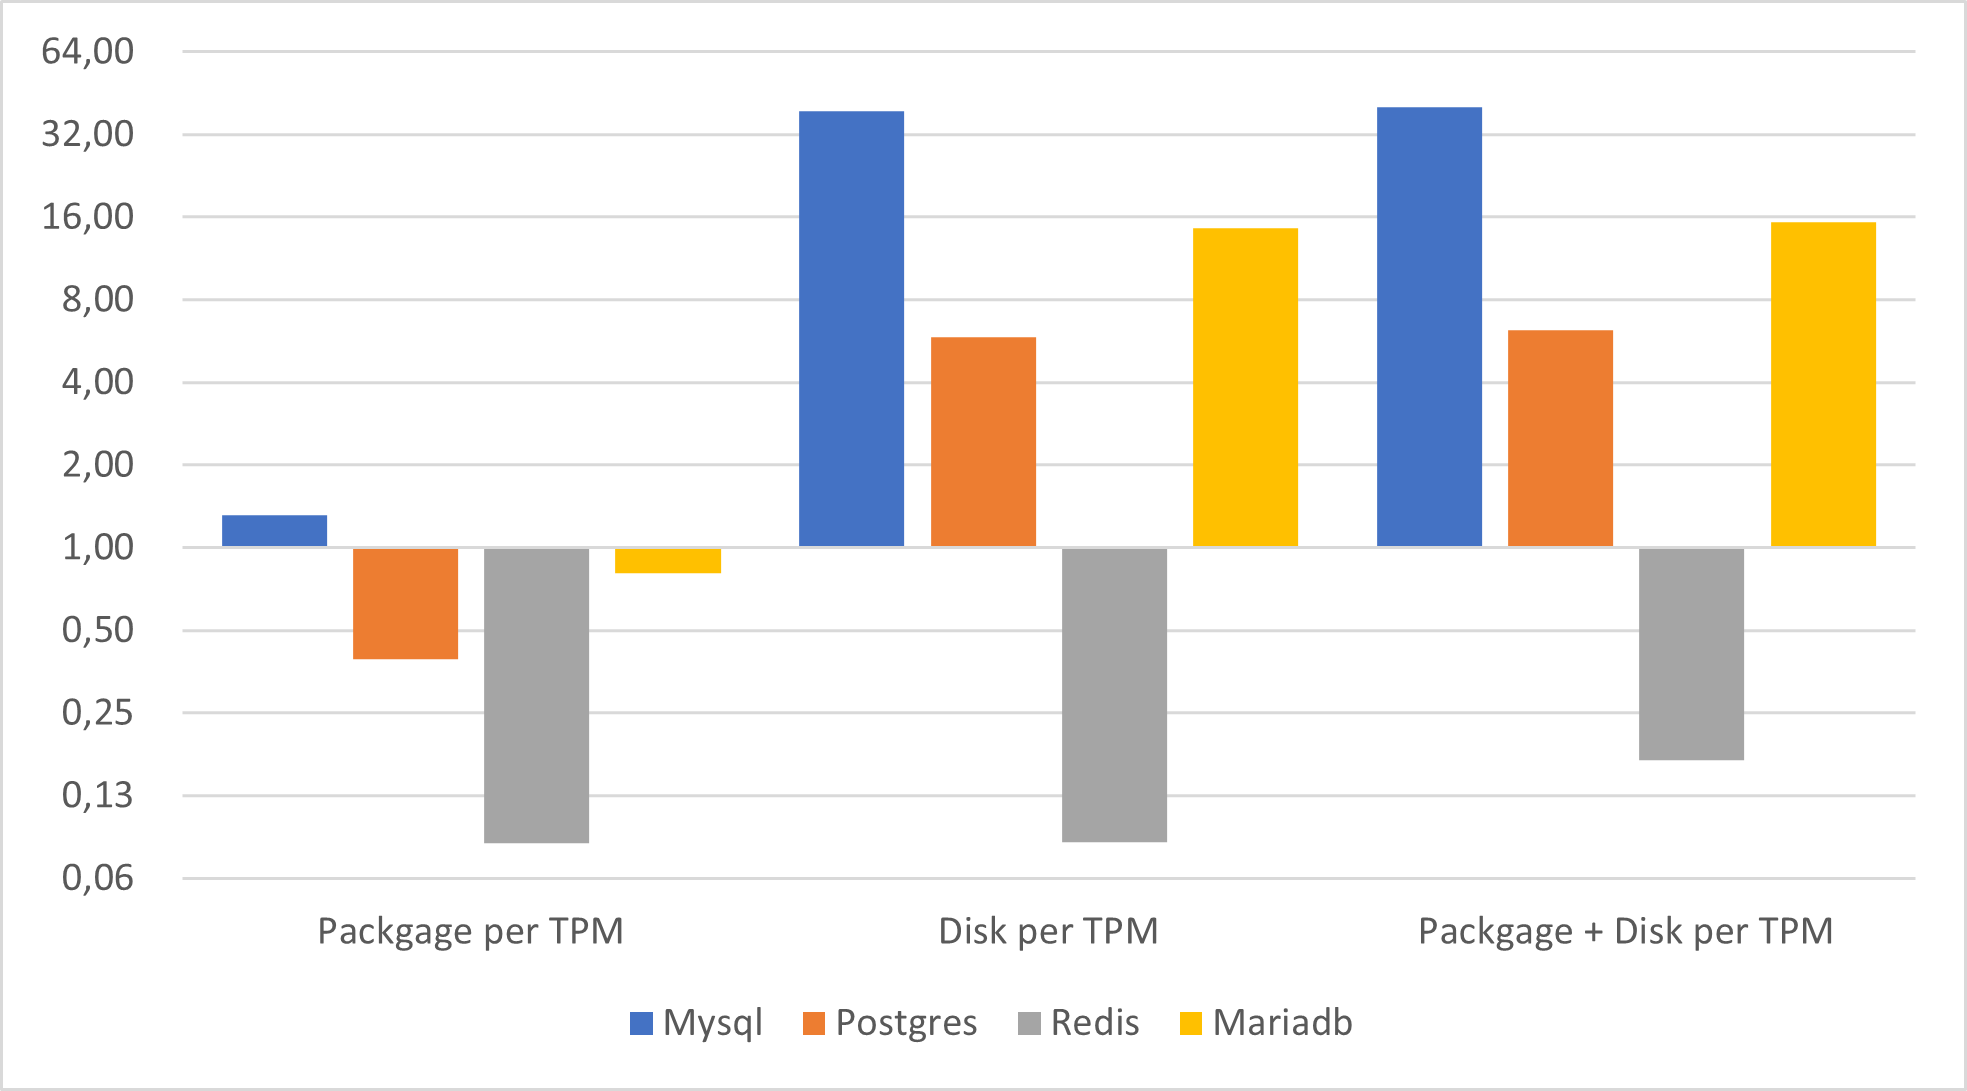
\includegraphics[width=0.8\columnwidth]{results/median/energy-tpm.png}
\caption{Median of energy consumption per TPM}
\label{fig:mediantpmenergy}
\end{figure}




\begin{figure}[!ht]
        \centering
        \begin{subfigure}[b]{0.30\textwidth}
            \centering
			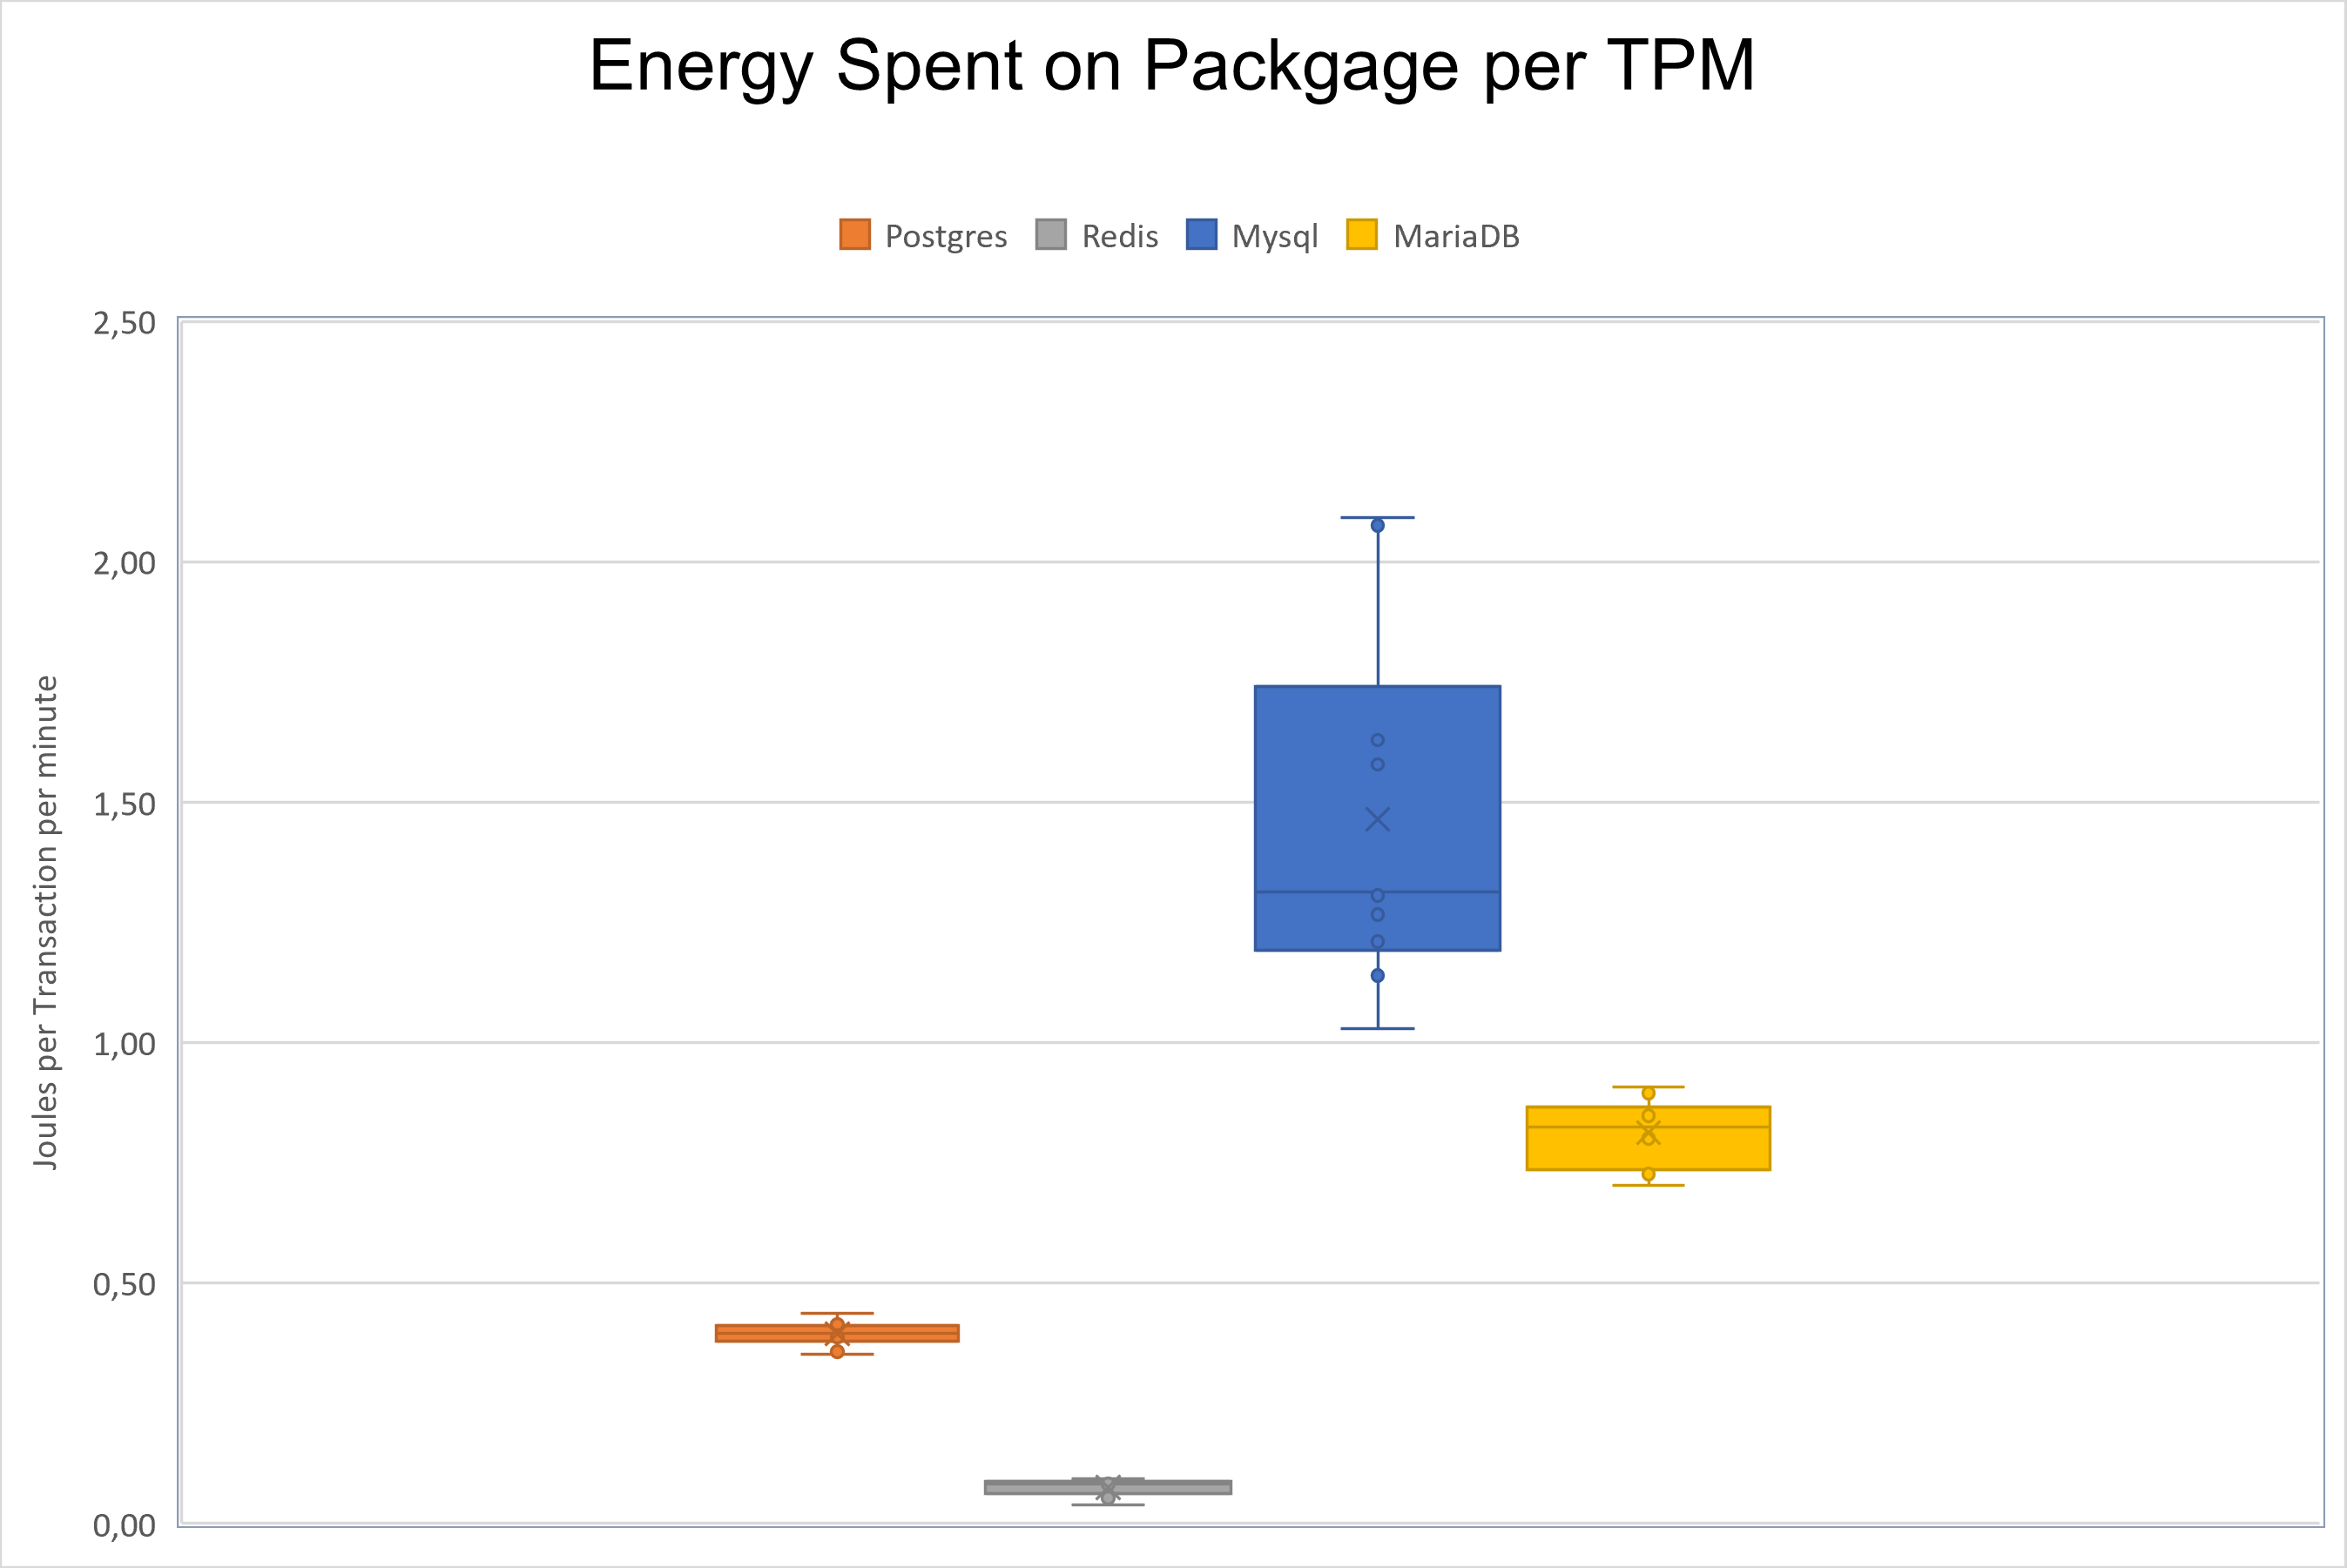
\includegraphics[width=1\columnwidth]{results/boxplot/Packgage-tpm.png}
			\caption[]%
            {{\small Energy consumption on Package per TPM}}    
			\label{fig:bocplottranspackage}
        \end{subfigure}
        \begin{subfigure}[b]{0.30\textwidth}  
            \centering 
            \includegraphics[width=1\columnwidth]{results/boxplot/Disk-tpm.png}
            \caption[]%
            {{\small Energy consumption on Disk per TPM}}    
            \label{fig:bocplottransdisk}
        \end{subfigure}
        \begin{subfigure}[b]{0.30\textwidth}  
            \centering 
            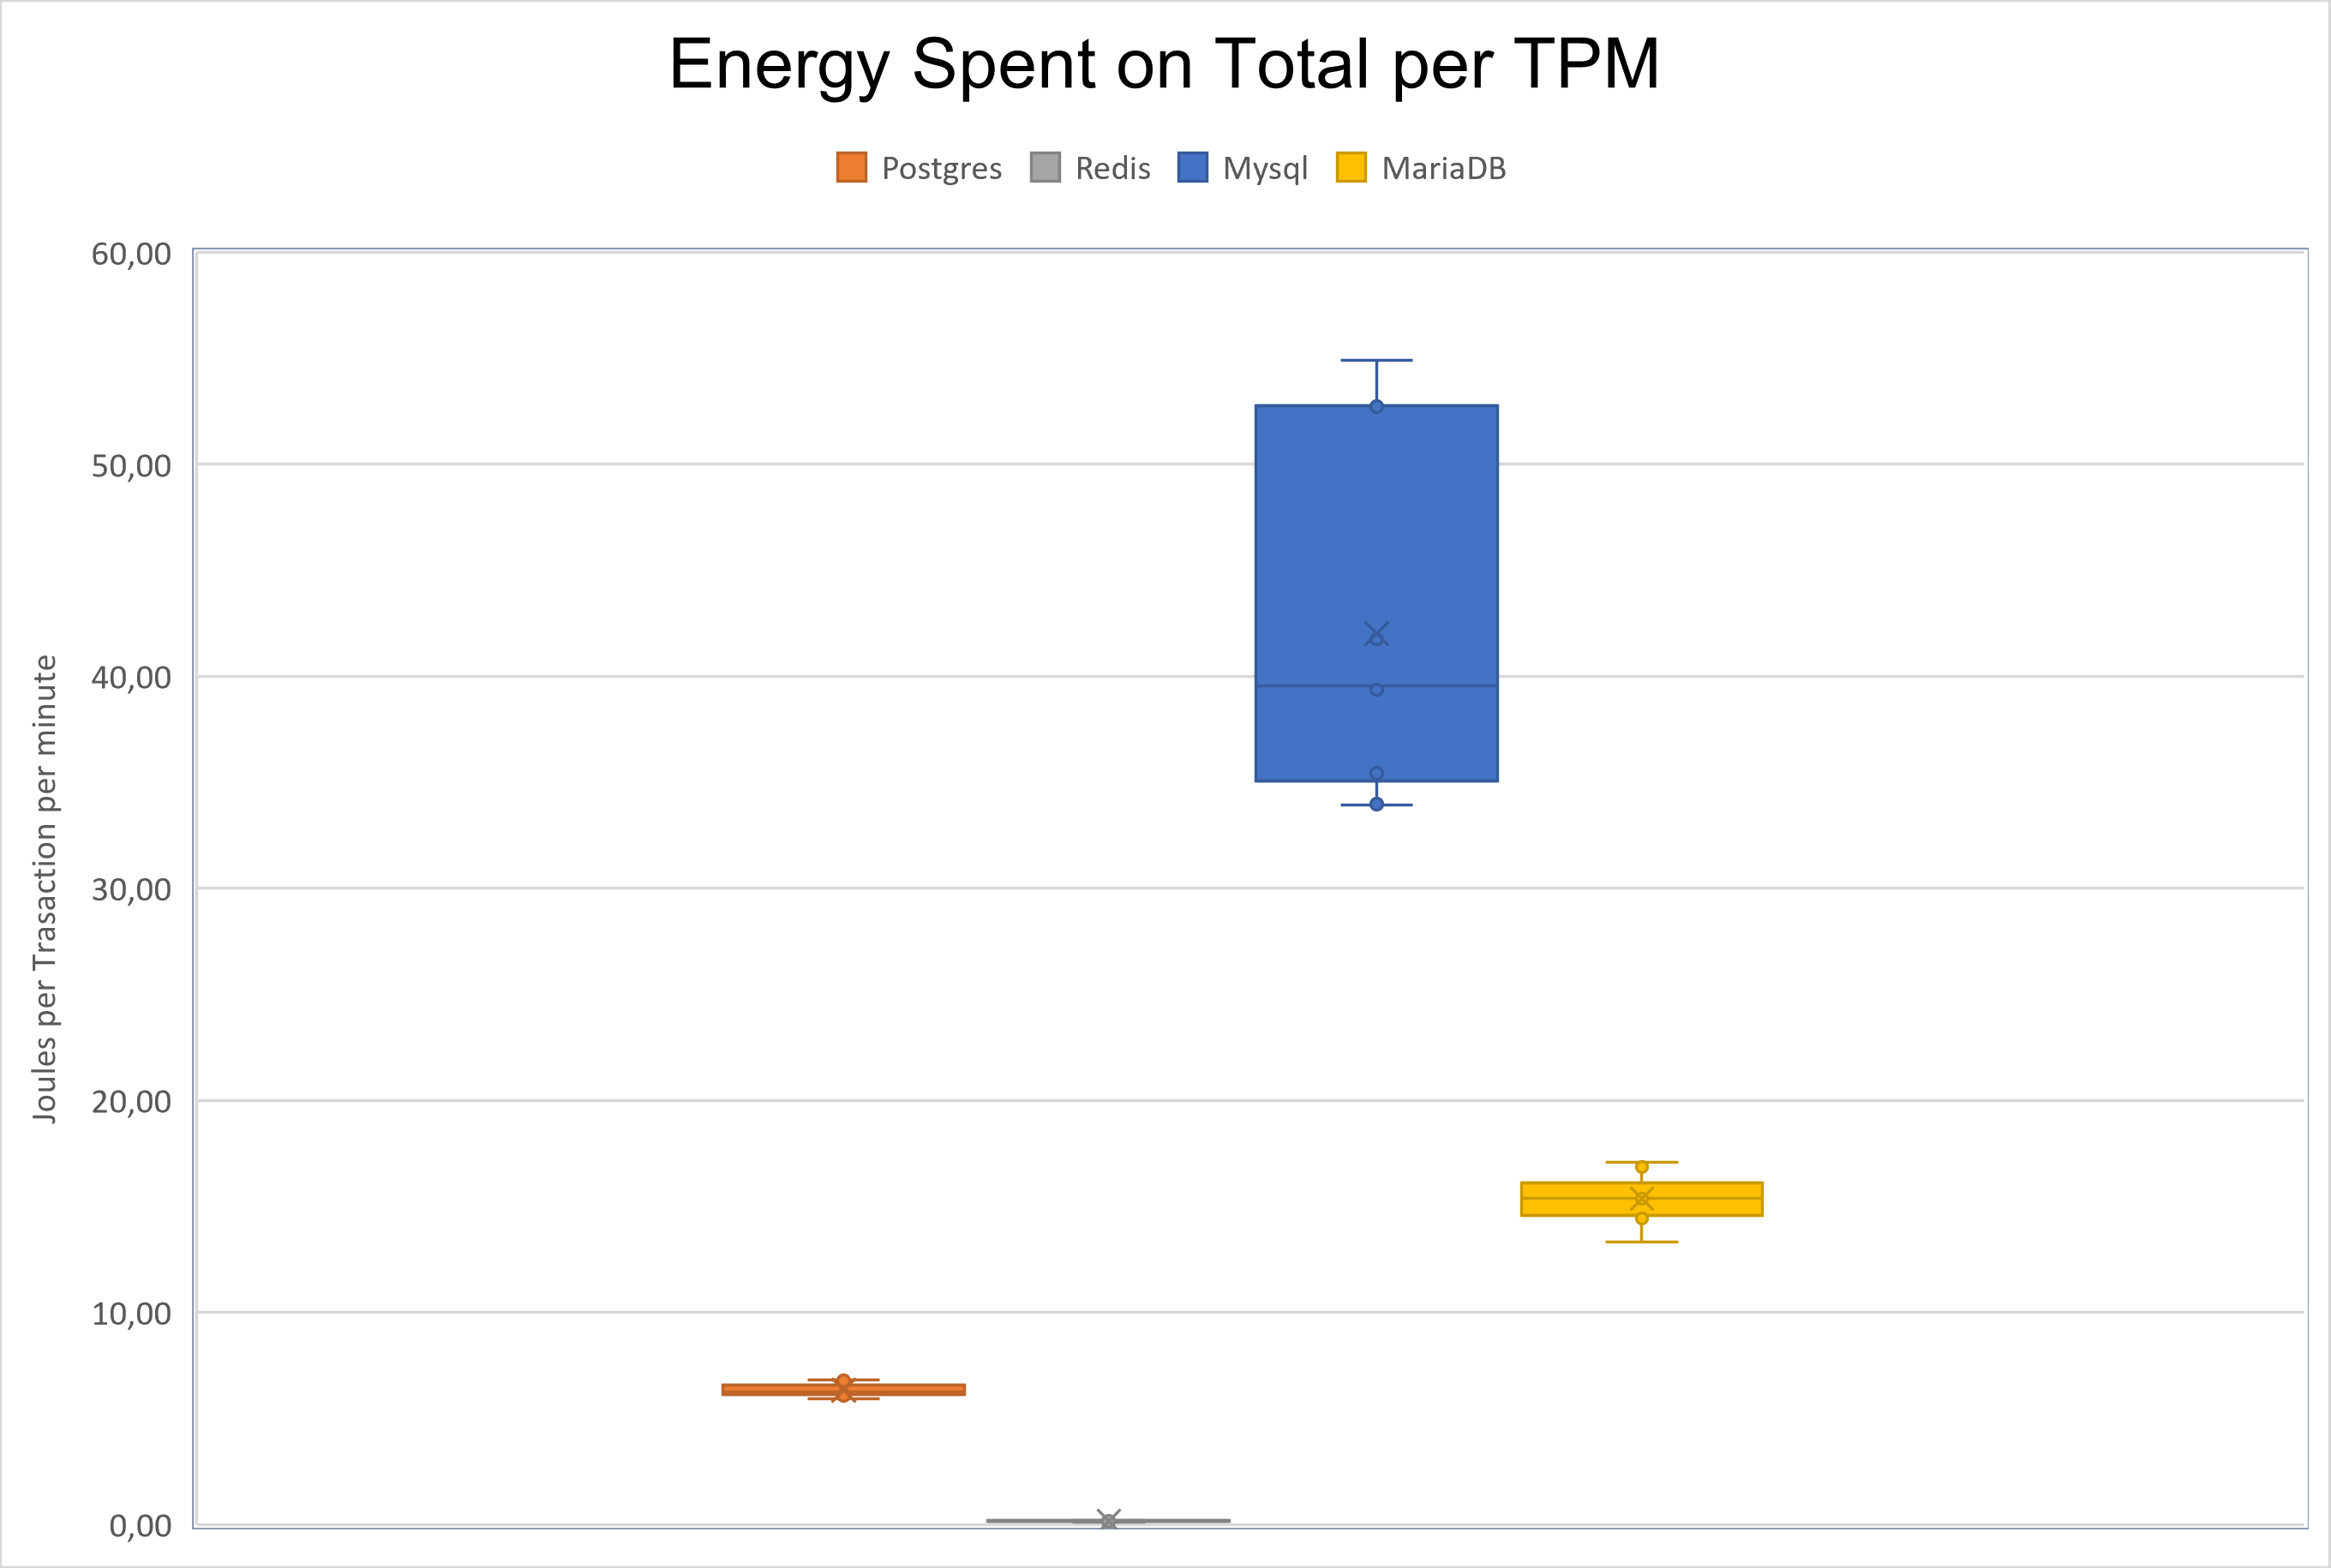
\includegraphics[width=1\columnwidth]{results/boxplot/total-tpm.png}
            \caption[]%
            {{\small Energy consumption on Overall System per TPM}}    
            \label{fig:bocplottranstotal}
        \end{subfigure}
        \caption[ Distribution of Energy consumption per TPM  ]
        {\small Distribution Energy consumption per TPM } 
        \label{fig:bocplottrans}
    \end{figure}
   


    In terms of Joules per \gls{nopm}, we can see the median in Figure \ref{fig:mediannopmenergy} that in the package the one with the most \gls{nopm} per Joules is Redis then MySQL, MariaDB, and Postgres. On the disk the one with the most Joules per \gls{nopm} is MySQL then MariaDB, Redis, and finally Postgres. When talking of the system as a whole the MySQL is the one with the Joules per \gls{nopm}, follow by MariaDB, Redis, and Postgres. This result doesn't follow any trend of the rational database being the most expensive or non relational database being the less expensive in any of the cases.

\begin{figure}[H]
\centering
    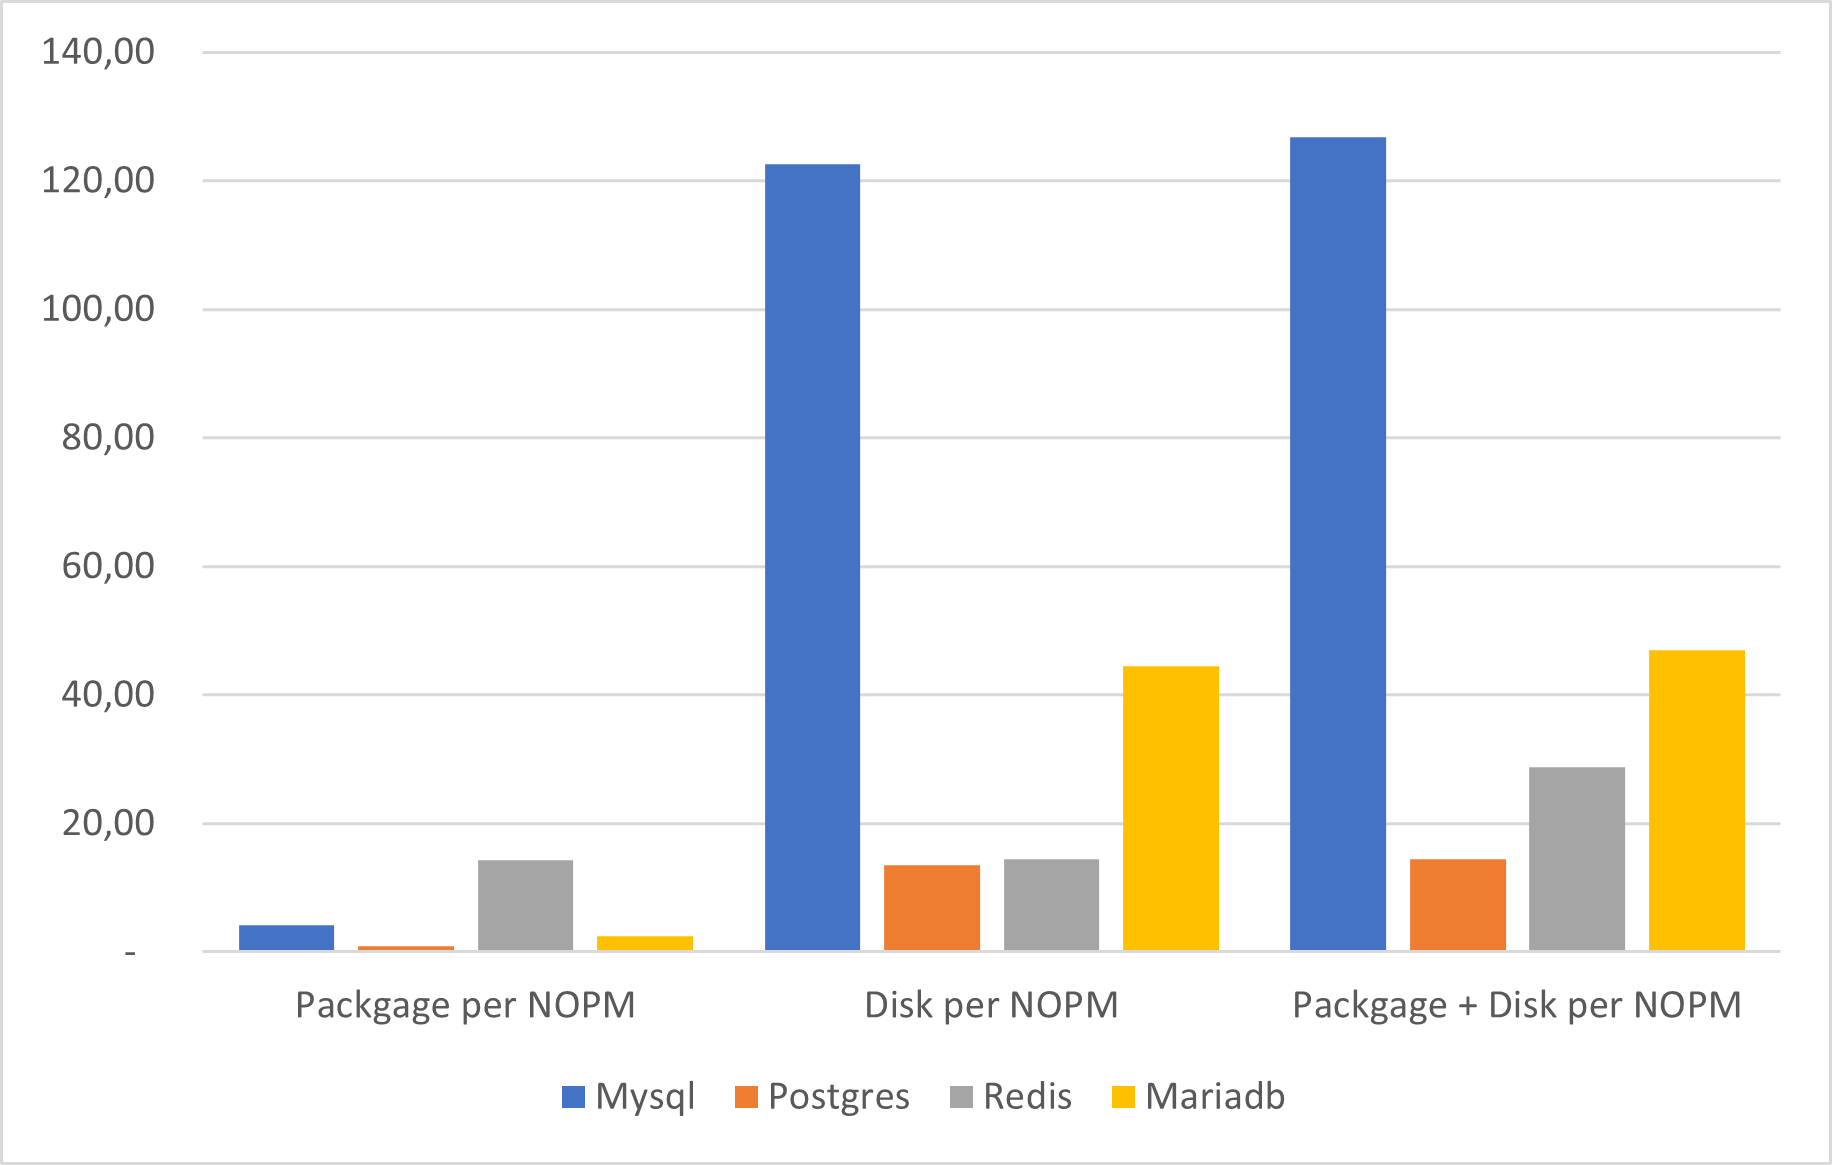
\includegraphics[width=0.8\columnwidth]{results/median/energy-nopm.png}
\caption{Median of energy consumption per NOPM}
\label{fig:mediannopmenergy}\end{figure}


\begin{figure}[!ht]
        \centering
        \begin{subfigure}[b]{0.32\textwidth}
            \centering
			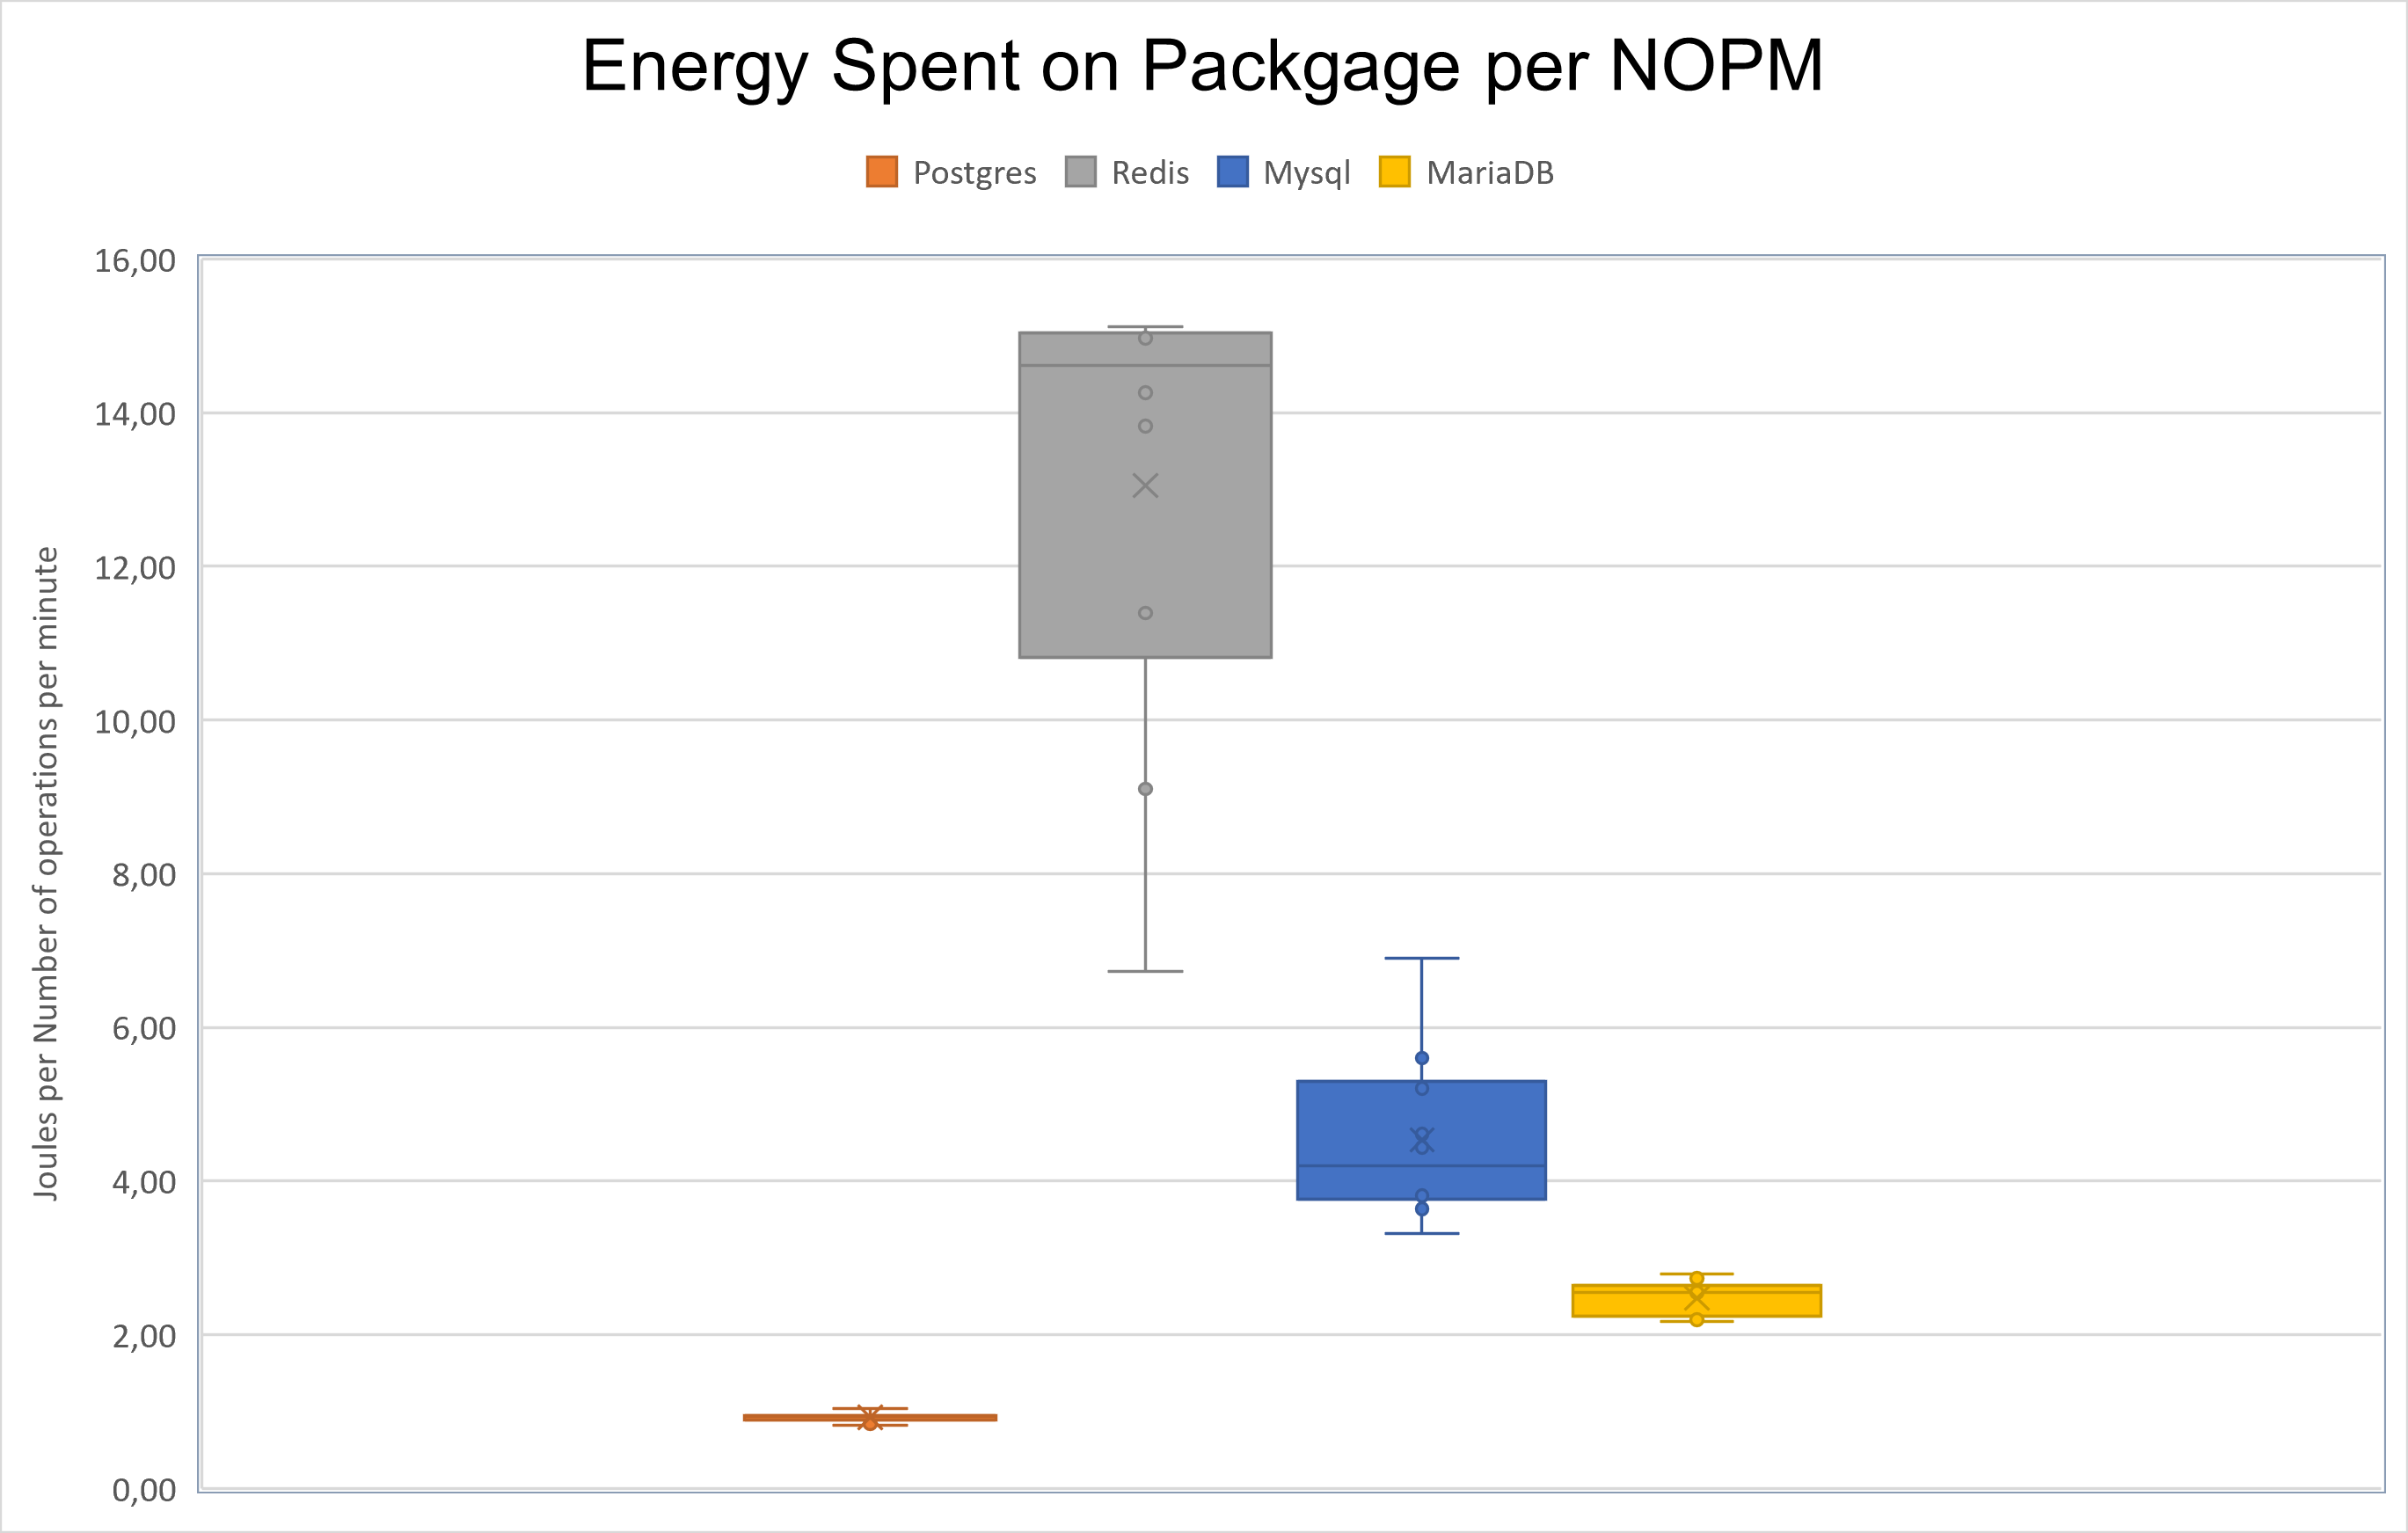
\includegraphics[width=1\columnwidth]{results/boxplot/Packgage-nopm.png}
			\caption[]%
            {{\small Energy consumption on Package per NOPM}}    
			\label{fig:bocplotnopmpackage}
        \end{subfigure}
        \begin{subfigure}[b]{0.32\textwidth}  
            \centering 
            \includegraphics[width=1\columnwidth]{results/boxplot/Disk-nopm.png}
            \caption[]%
            {{\small Energy consumption on Disk per NOPM}}    
            \label{fig:bocplotnopmdisk}
        \end{subfigure}
        \begin{subfigure}[b]{0.32\textwidth}  
            \centering 
                \includegraphics[width=1\columnwidth]{results/boxplot/total-nopm.png}
            \caption[]%
            {{\small Energy consumption on Overall System per NOPM}}    
            \label{fig:bocplotnopmtotal}
        \end{subfigure}
        \caption[ Distribution of energy consumption per NOPM ]
        {\small Distribution of energy consumption per NOPM} 
        \label{fig:bocplotnumber}
    \end{figure}
   





\subsection{DBMS in Multi User: Energy Consumption}

%Finally, for the multi users, a different approach was made
 %here, where in Figure \ref{fig:vuyenergy} shows the evolution of energy consumption (Y-axis) on Package, CPU, Disk and global system with the different numbers of virtual users (X-axis), in Figure \ref{fig:vuhammer} shows the evolution of the performance of \gls{tpm} and \gls{nopm} with the different number virtual users and in Figures \ref{fig:vuyenergytpm} and \ref{fig:vuyenergynopm}  shows the evolution of \gls{tpm} and \gls{nopm} per Joules with the different users.





\paragraph{Energy Consumption with Multi Users}


    Now for the Multi users, we will first be discussing the energy consumption on Package as shown in Figure \ref{fig:vuyenergypackage}.  Redis is the only one with slightly different behavior with an increase of users where the other three DBMS had a rise of energy consumption, also Redis has decreased with eight users followed by a rise with 32 users follow by another drastic decrease. Also noted that of the relational DBMS, MariaDB is the one with more increase, and MySQL is the one with the lowest increase.

    In Figure \ref{fig:vuyenergydisk} can be seen the energy consumption on disk with an increase of users. MariaDB has an noticeable increase, Postgres also has an increase, MySQL and Redis has a improvement in energy consumption. And with these variations of users, the MariaDB become the most expensive followed by Postgres, MySQL, and Redis.
    
    On a general view, Redis has the same pattern as in the disk being the lowest in terms of energy consumption except on 32 users, where the increase in Package has a large impact on the overall energy and putting him in the second-lowest behind MySQL. MySQL  starts as the highest and with the increase becomes the second-lowest energy consumption \gls{dbms} expect on 32 users where he is the lowest. Postgres is second highest. Finally, MariaDB with the increase of users become the most expensive \gls{dbms}.
    
    The only conclusion that can maybe be drawn here is that Redis has an increase in energy efficiency that can be possible due to its nature as a non-relational database with data in memory.

   \begin{figure}[!ht]
        \centering
        \begin{subfigure}[b]{0.45\textwidth}
            \centering
			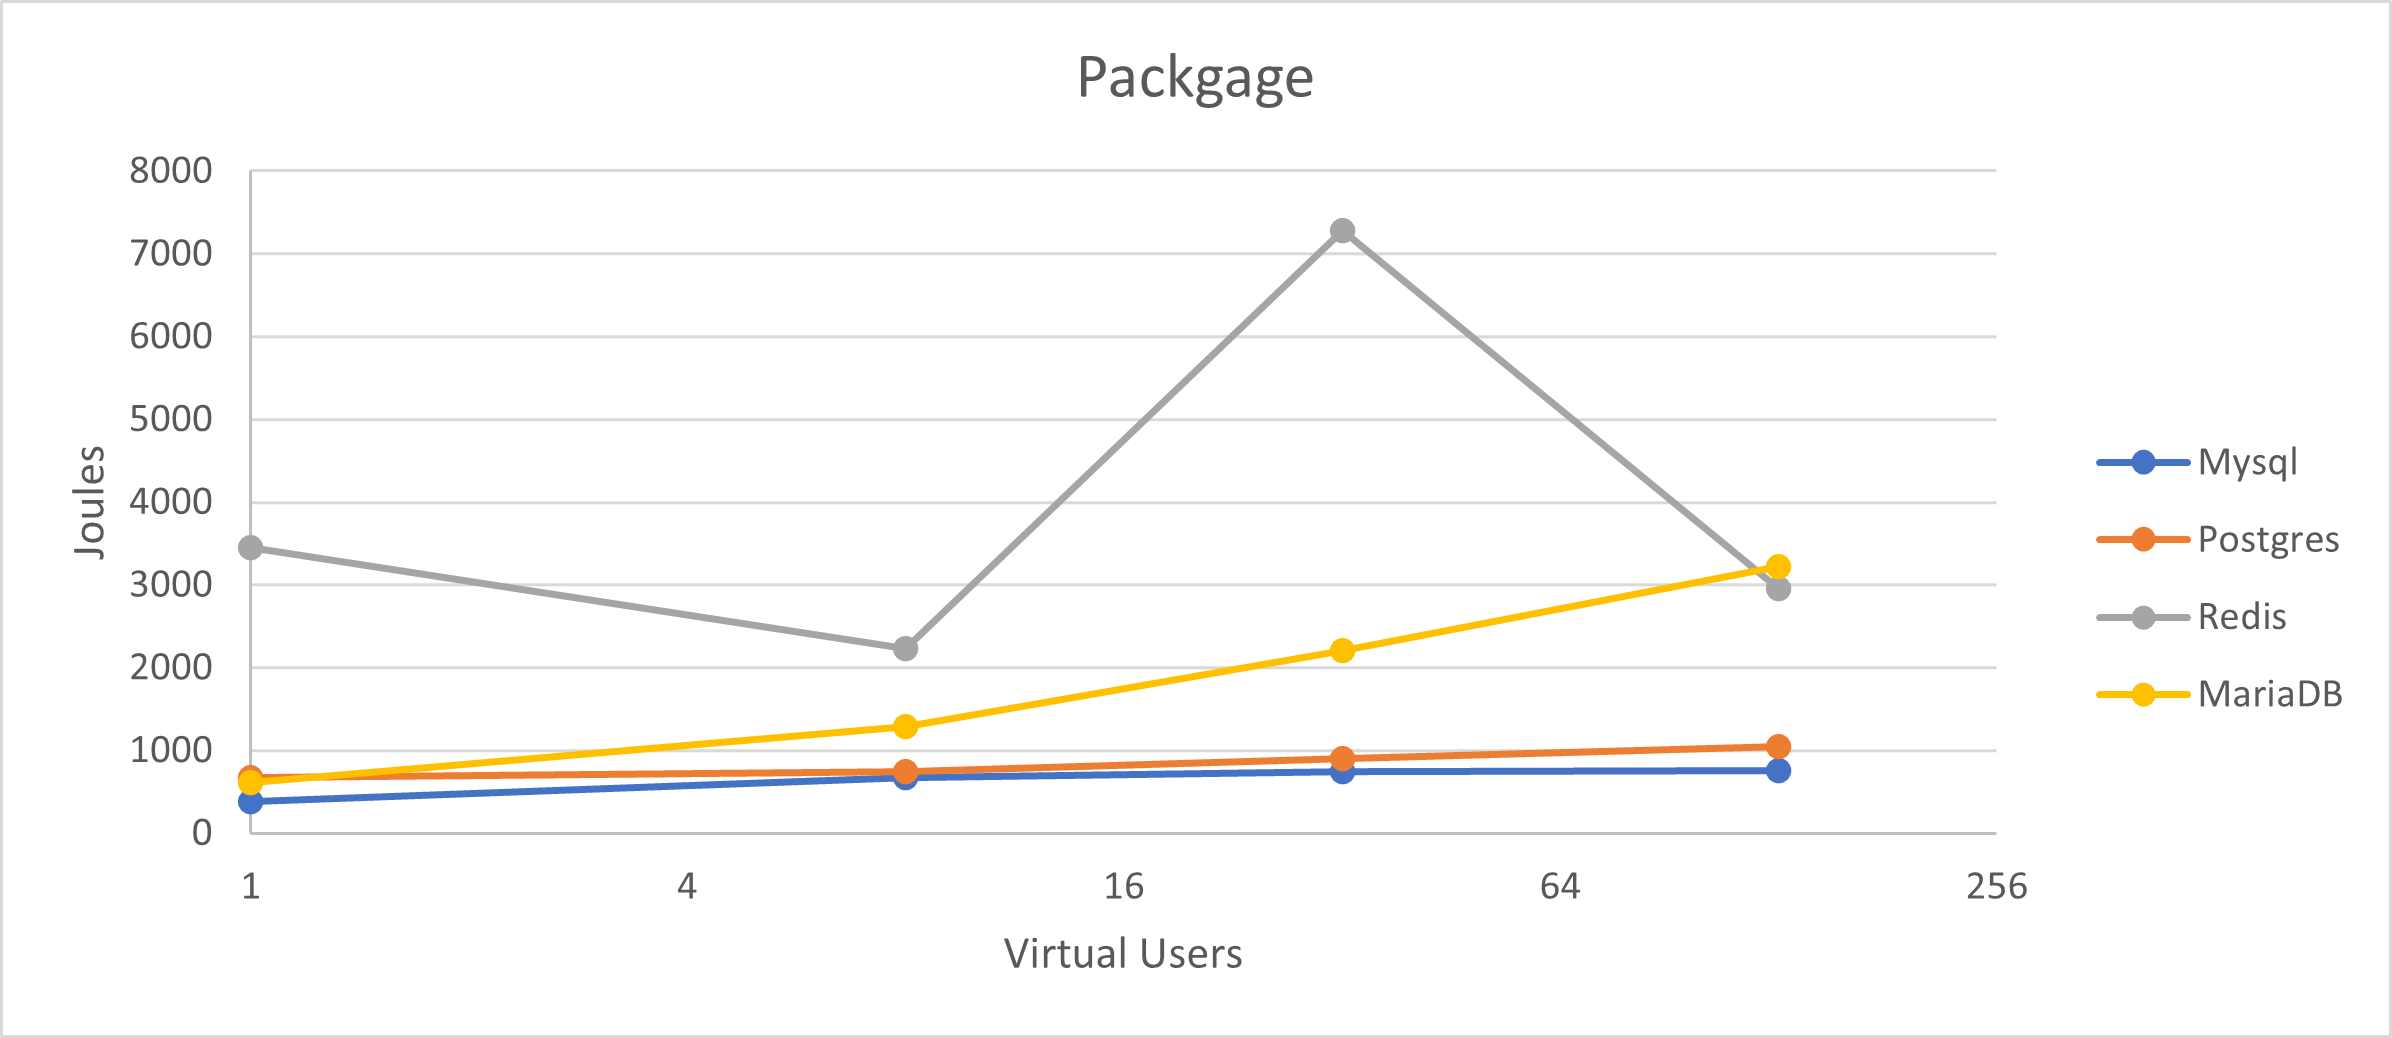
\includegraphics[width=1\columnwidth]{results/vu/Packgage.png}
			\caption[]%
            {{\small Energy consumption on Package with different number of users}}
			\label{fig:vuyenergypackage}
        \end{subfigure}
        \hfill
        \begin{subfigure}[b]{0.45\textwidth}  
            \centering 
            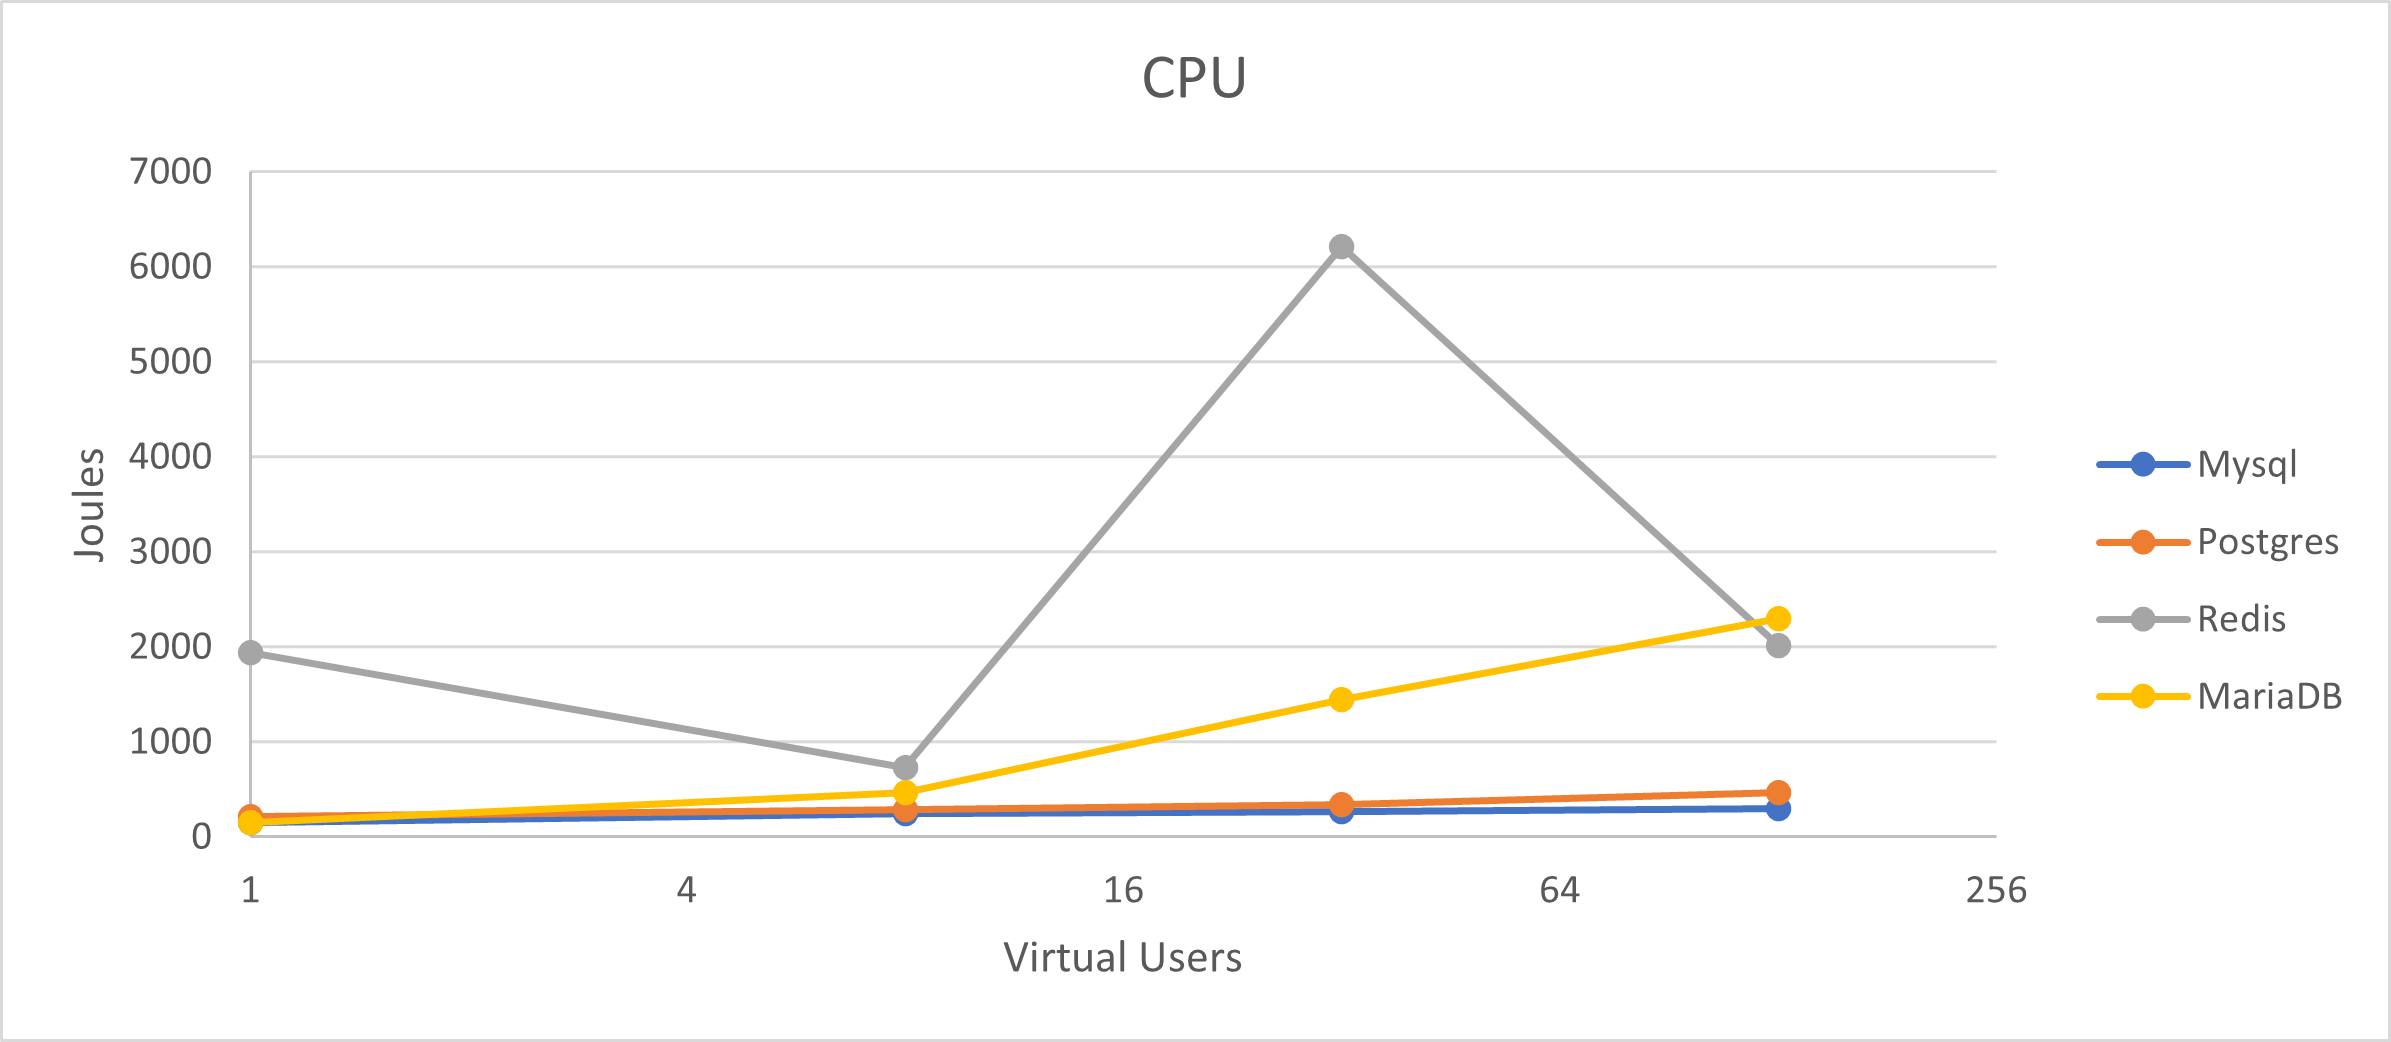
\includegraphics[width=1\columnwidth]{results/vu/CPU.png}
            \caption[]%
            {{\small Energy consumption on CPU with different number of users}}
            \label{fig:vuyenergycpu}
        \end{subfigure}
        \vskip\baselineskip
        \begin{subfigure}[b]{0.45\textwidth}   
            \centering 
            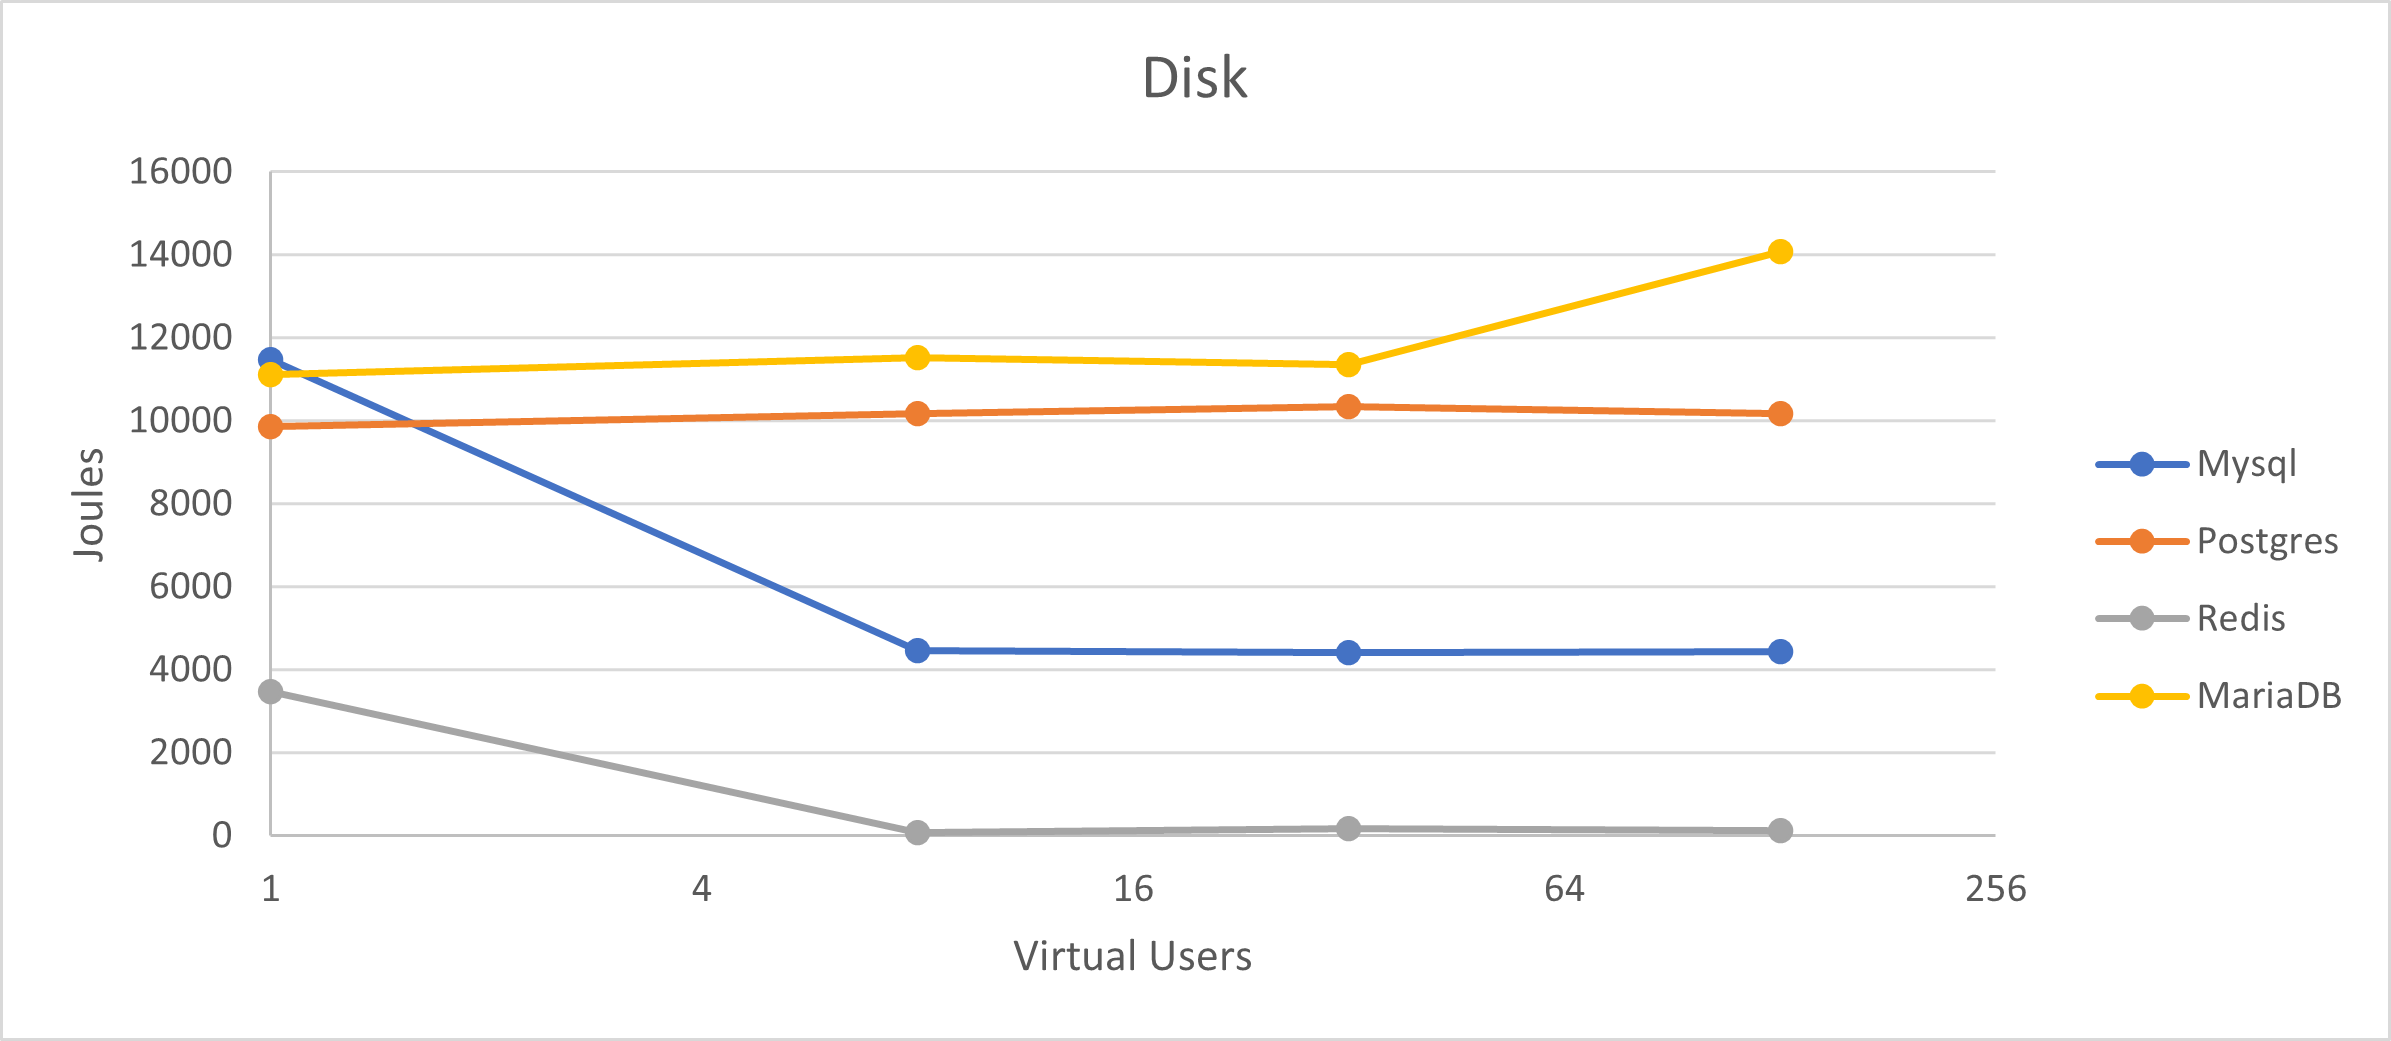
\includegraphics[width=1\columnwidth]{results/vu/Disk.png}
            \caption[]%
            {{\small Energy consumption on Disk with different number of users}}
            \label{fig:vuyenergydisk}
        \end{subfigure}
        \hfill
        \begin{subfigure}[b]{0.45\textwidth}   
            \centering 
			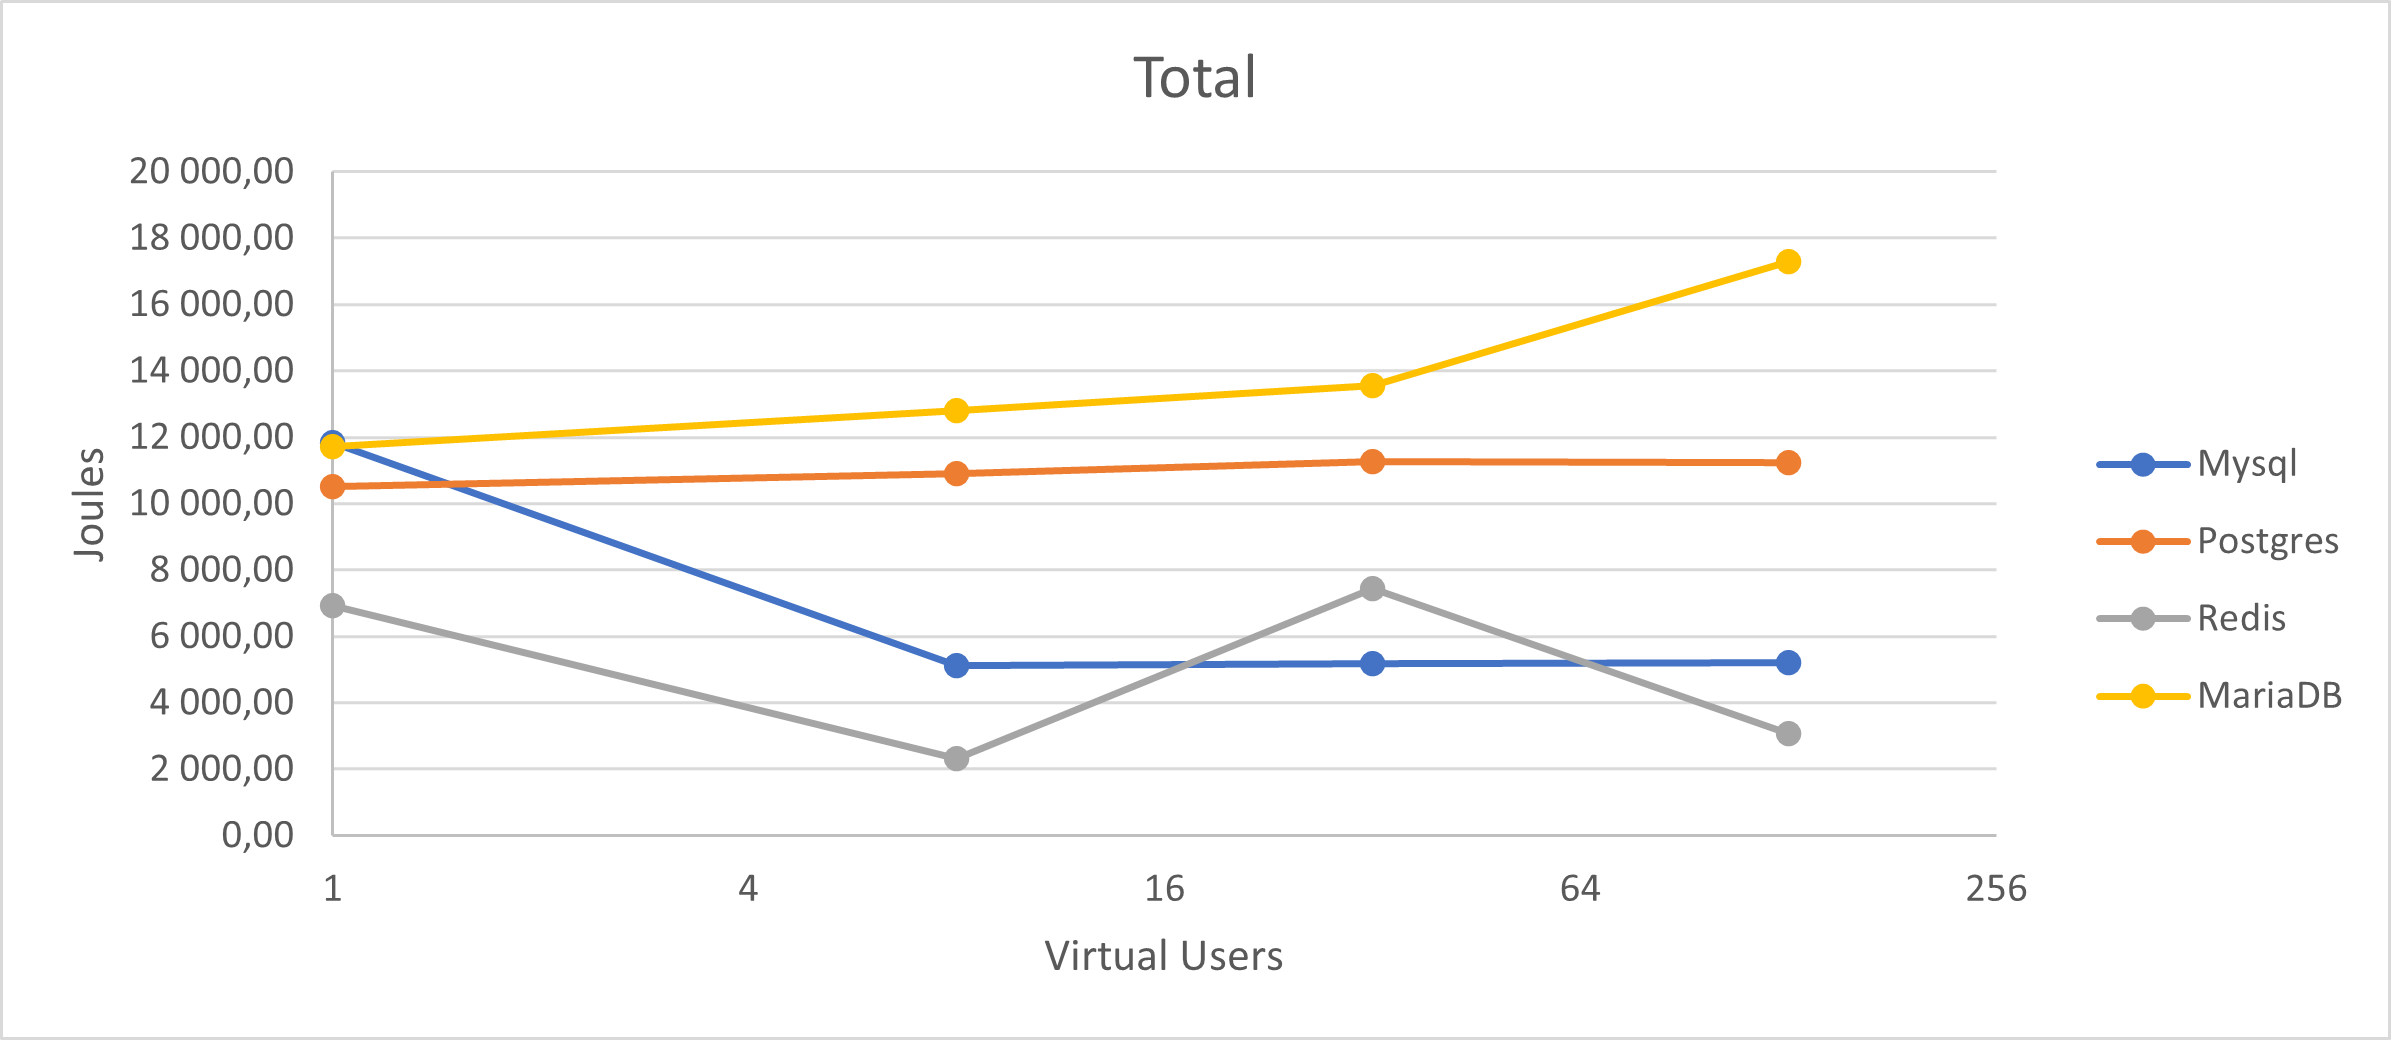
\includegraphics[width=1\columnwidth]{results/vu/Total.png}
            \caption[]%
            {{\small Energy consumption on Overall System with different number of users}}
            \label{fig:vuyenergytotal}
        \end{subfigure}
        \caption[ Energy consumption with different number of users ]
        {\small Energy consumption with different number of users} 
        \label{fig:vuyenergy}
    \end{figure}


\paragraph{Runtime Performance with Multi Users}

    When observing the performance of HammerDB benchmark with an increase of users, first can be seen that all \gls{dbms} had an increase of \gls{tpm} and \gls{nopm} with the variation of users. The only instance that had a decrease was from 32 to 128 users on Redis. With the increase of users, Redis still maintain the \gls{dbms} with better \gls{tpm} and \gls{nopm} and MySQL stays the worse, while Postgres with an increase of users start to get worse results comparing with MariaDB. This results are in Figure \ref{fig:vuhammerTPM} and Figure \ref{fig:vuhammerNOPM}.
    

       \begin{figure}[!ht]
        \centering
        \begin{subfigure}[b]{0.45\textwidth}
            \centering
			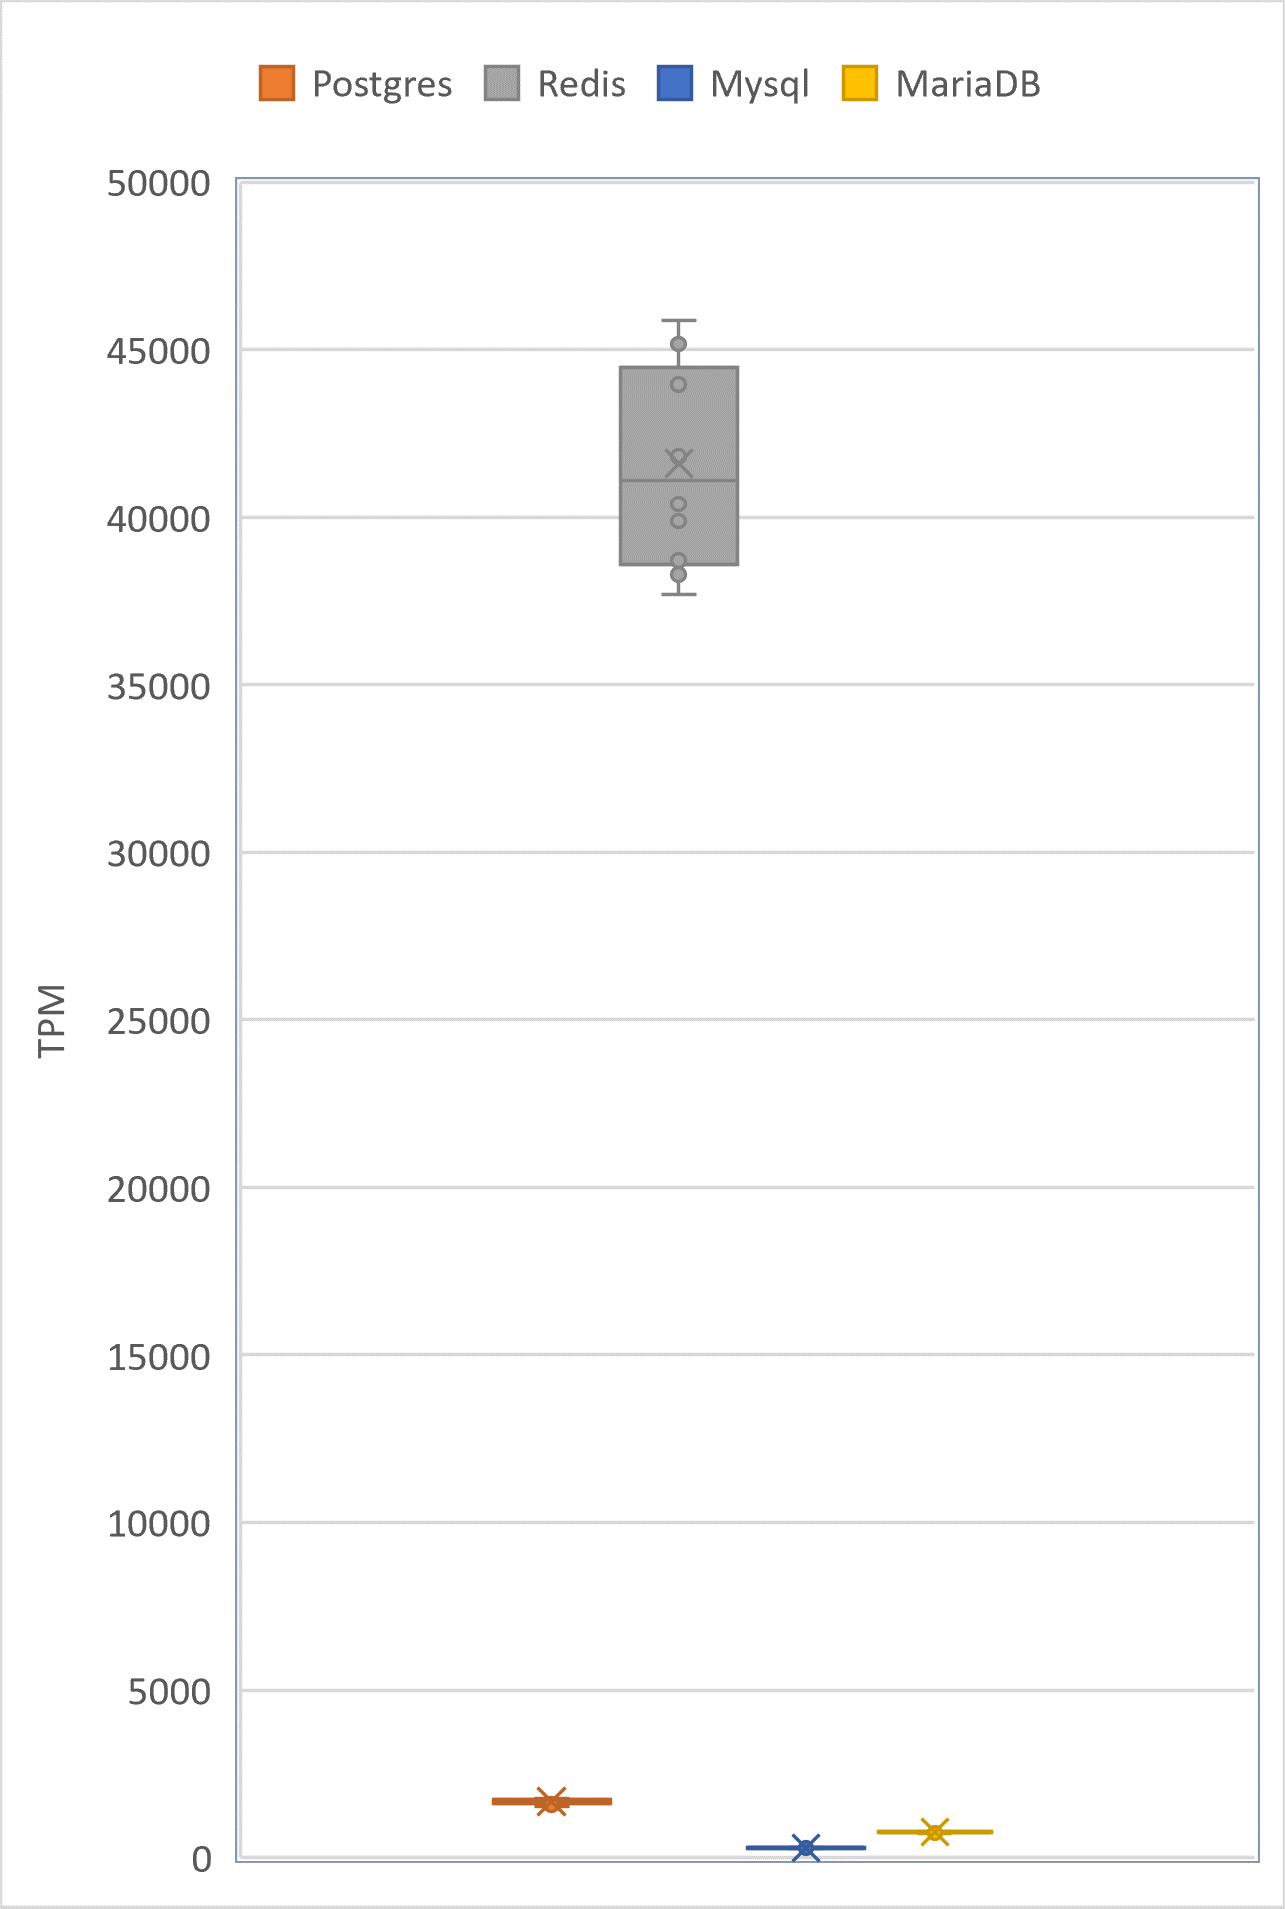
\includegraphics[width=1\columnwidth]{results/vu/TPM.png}
			\caption[]%
            {{\small TPM with different number of users}}    
			\label{fig:vuhammerTPM}
        \end{subfigure}
        \hfill
        \begin{subfigure}[b]{0.45\textwidth}  
            \centering 
            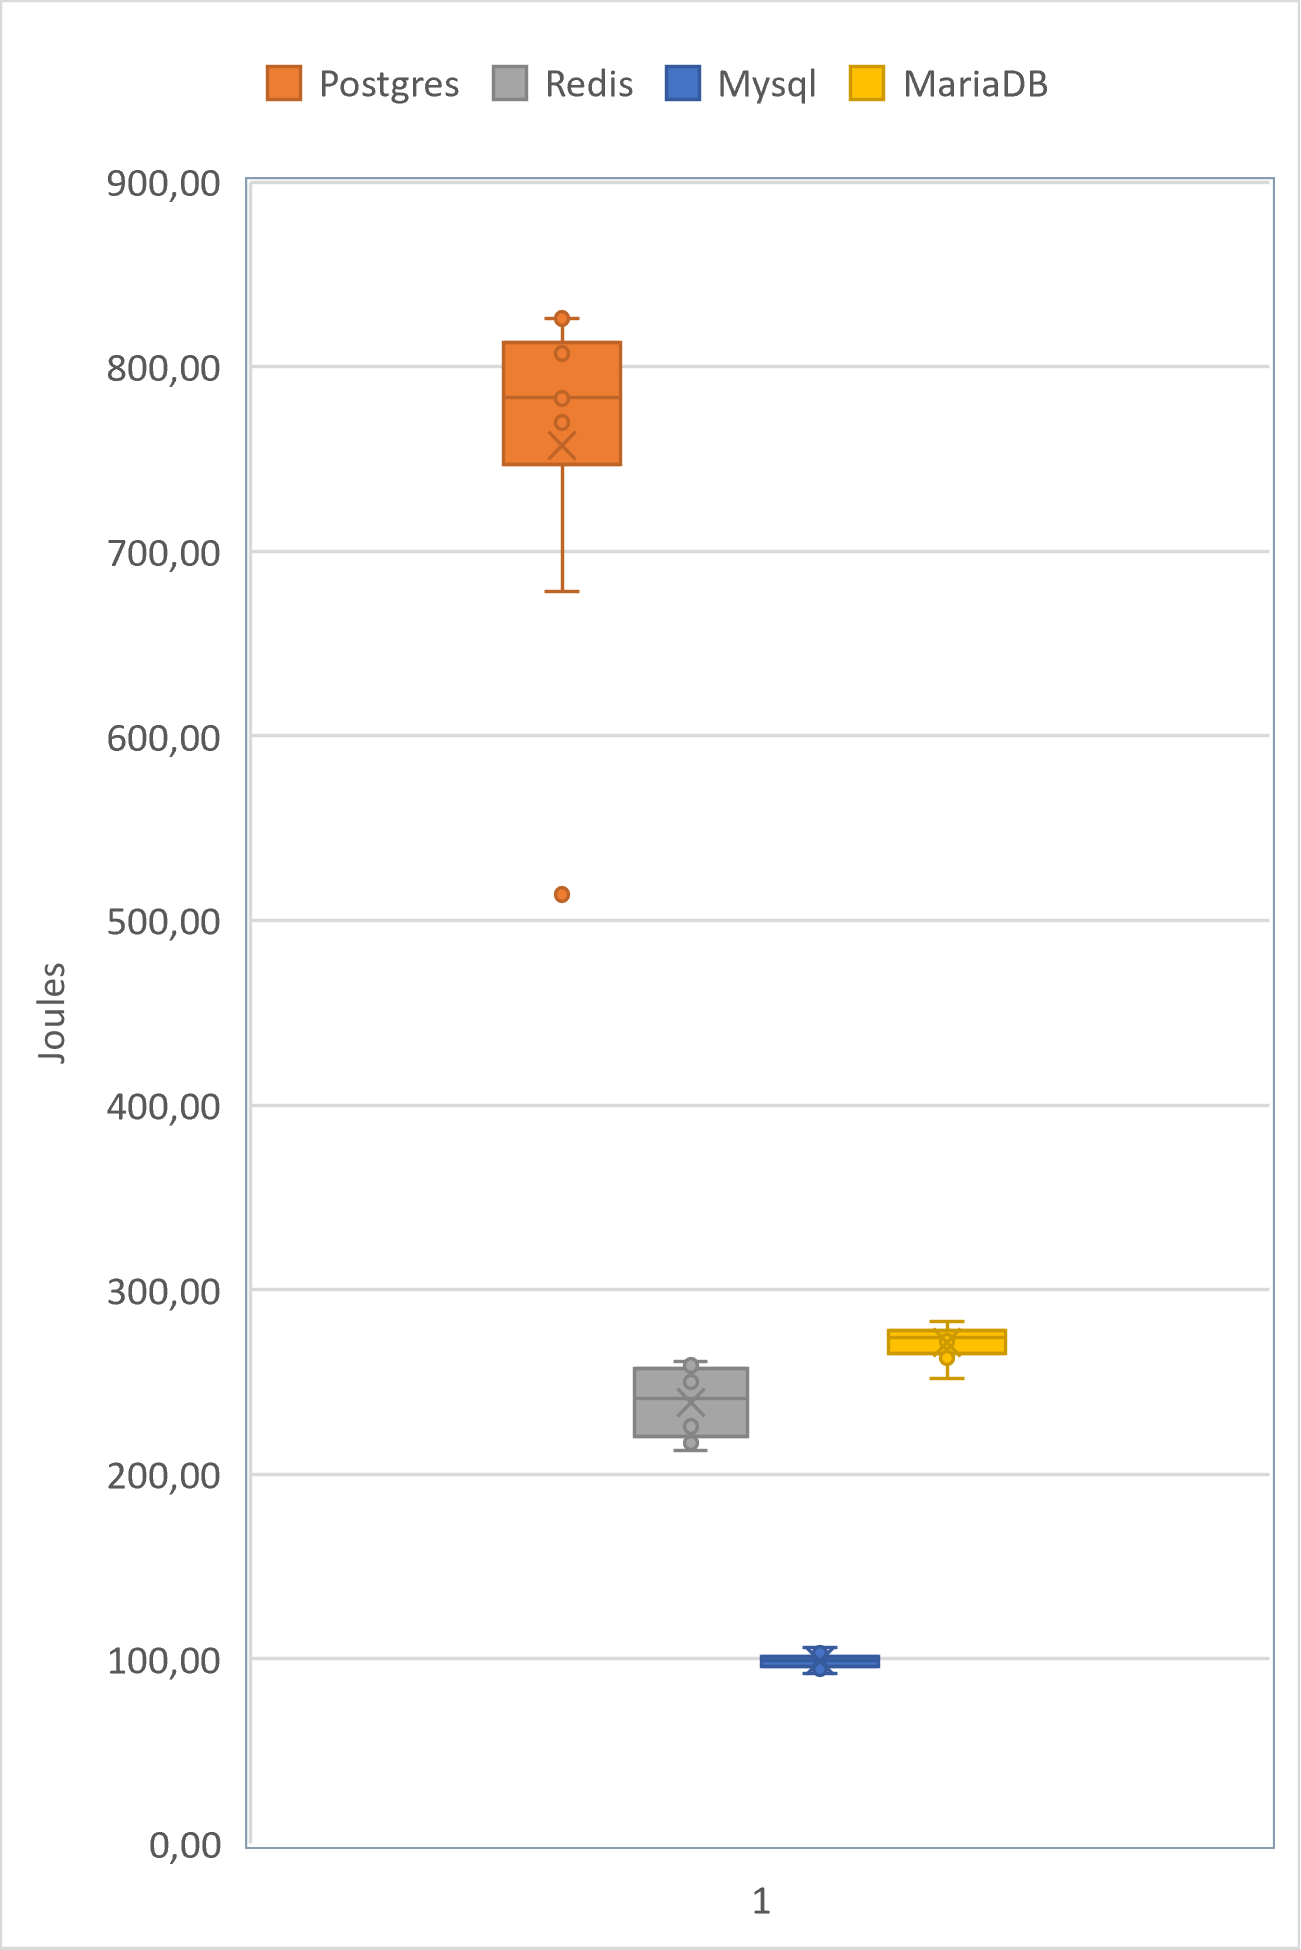
\includegraphics[width=1\columnwidth]{results/vu/NOPM.png}
            \caption[]%
            {{\small NOPM with different number of users}}    
            \label{fig:vuhammerNOPM}
        \end{subfigure}
        \vskip\baselineskip
        \caption[HammerDB results with different number of users]
        {\small HammerDB results with different number of users} 
        \label{fig:vuhammer}
    \end{figure}
   



\paragraph{Energy Consumption per Runtime Performance with Different Users}

    When discussing energy consumption per \gls{tpm} as seen in Figure \ref{fig:vuyenergytpm}, we can see with the increase of users that Redis have a better ratio in terms of energy per \gls{tpm}, and in general, all the databases except Postgres improved very well even though that MariaDB is the relational database with better results. These improvements happen because all \gls{dbms} except Postgres had a reduction of energy consumption on the disk per \gls{tpm} that provides a decrease in total energy consumption per \gls{tpm}. 
    
    \begin{figure}[h!]
        \centering
        \begin{subfigure}[b]{0.45\textwidth}
            \centering
			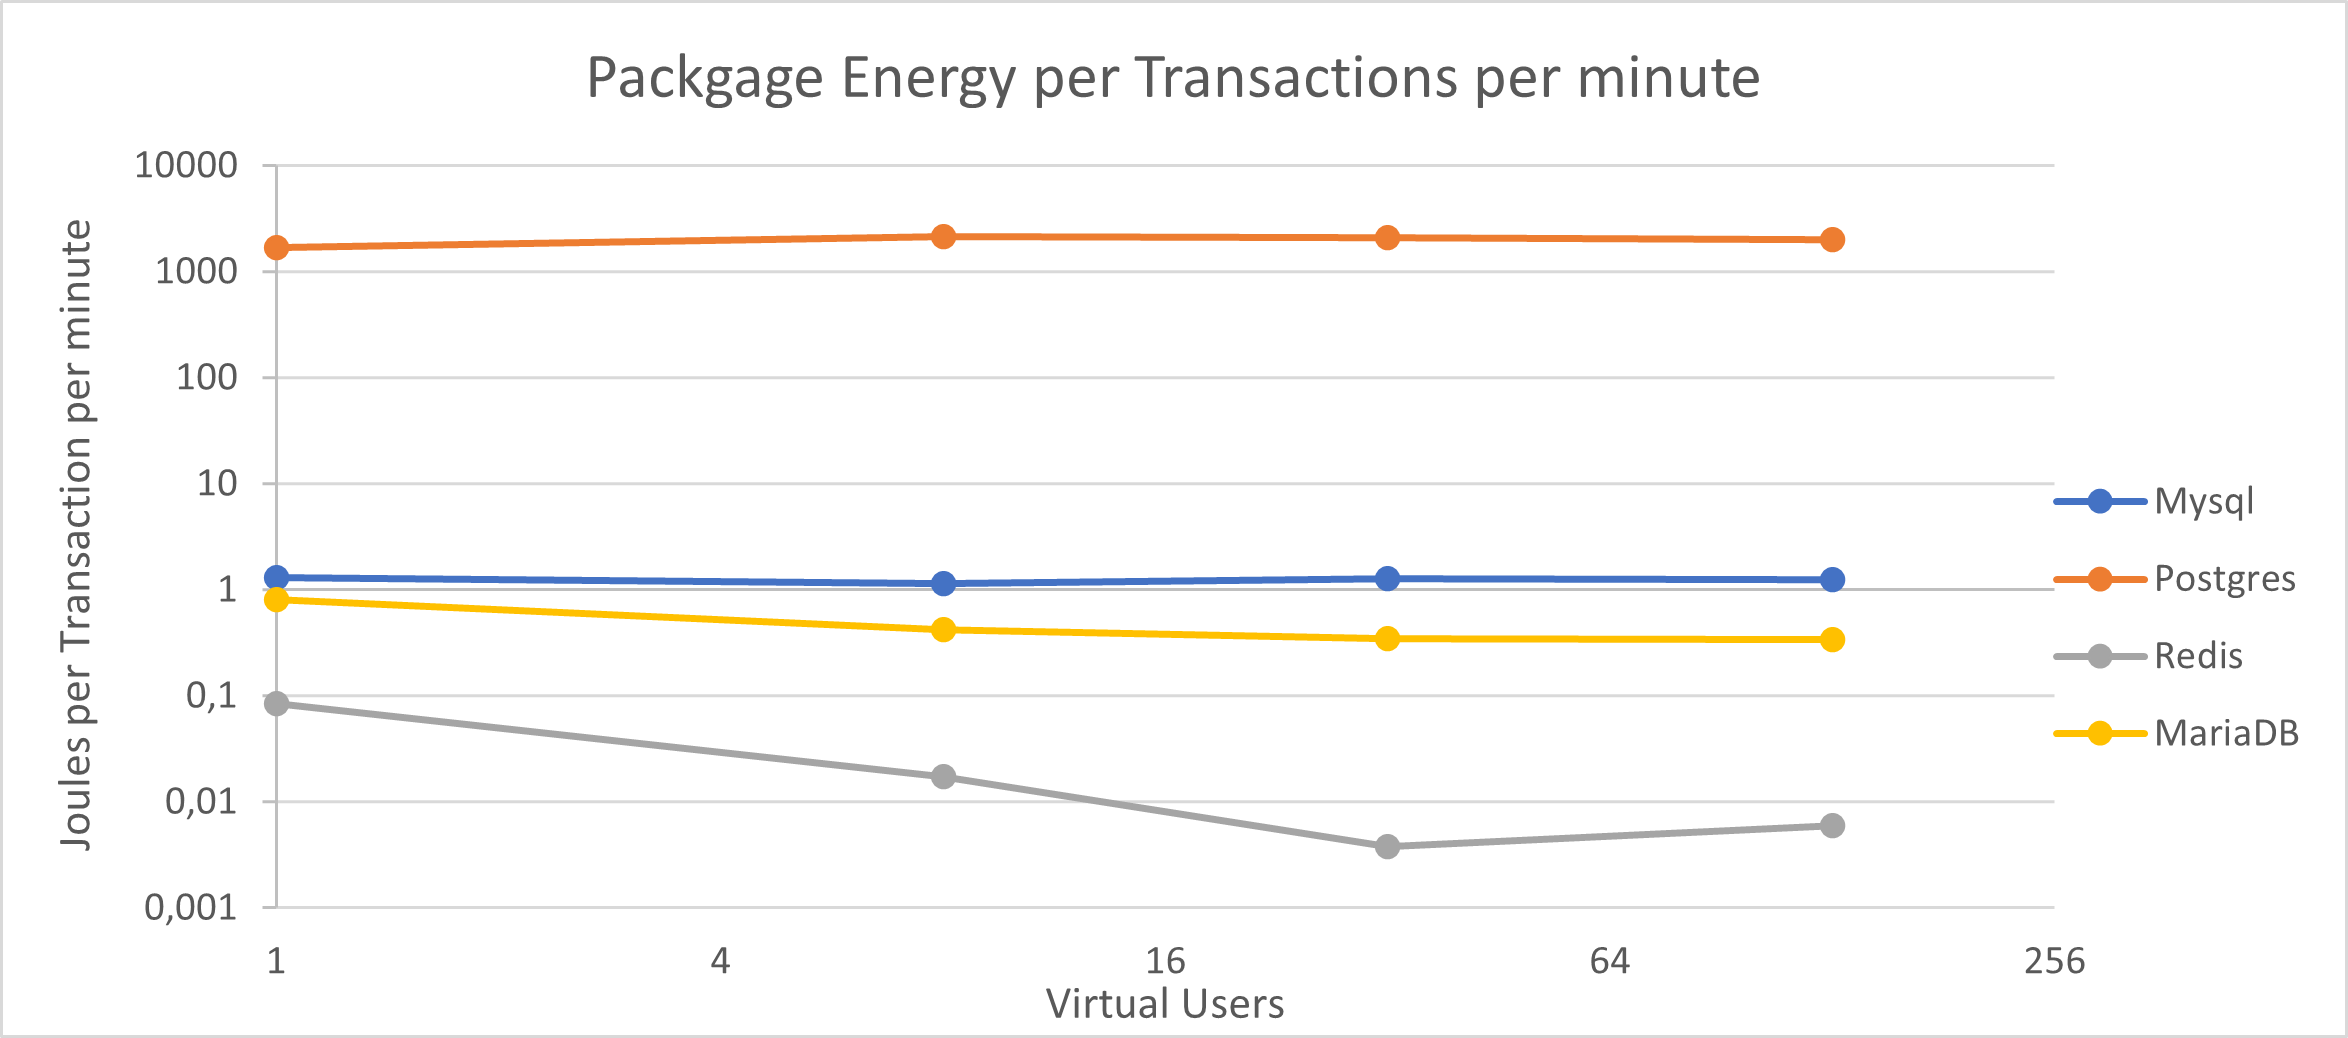
\includegraphics[width=1\columnwidth]{results/vu/package-tpm.png}
			\caption[]%
            {{\small Energy consumption on Package per TPM with different number users}}    
			\label{fig:vutranspackage}
        \end{subfigure}
        \hfill
        \begin{subfigure}[b]{0.45\textwidth}  
            \centering 
            \includegraphics[width=1\columnwidth]{results/vu/Disk-tpm.png}
            \caption[]%
            {{\small Energy consumption on Disk per TPM with different number users}}    
            \label{fig:vutransdisk}
        \end{subfigure}
        \vskip\baselineskip
        \begin{subfigure}[b]{0.45\textwidth}  
            \centering 
            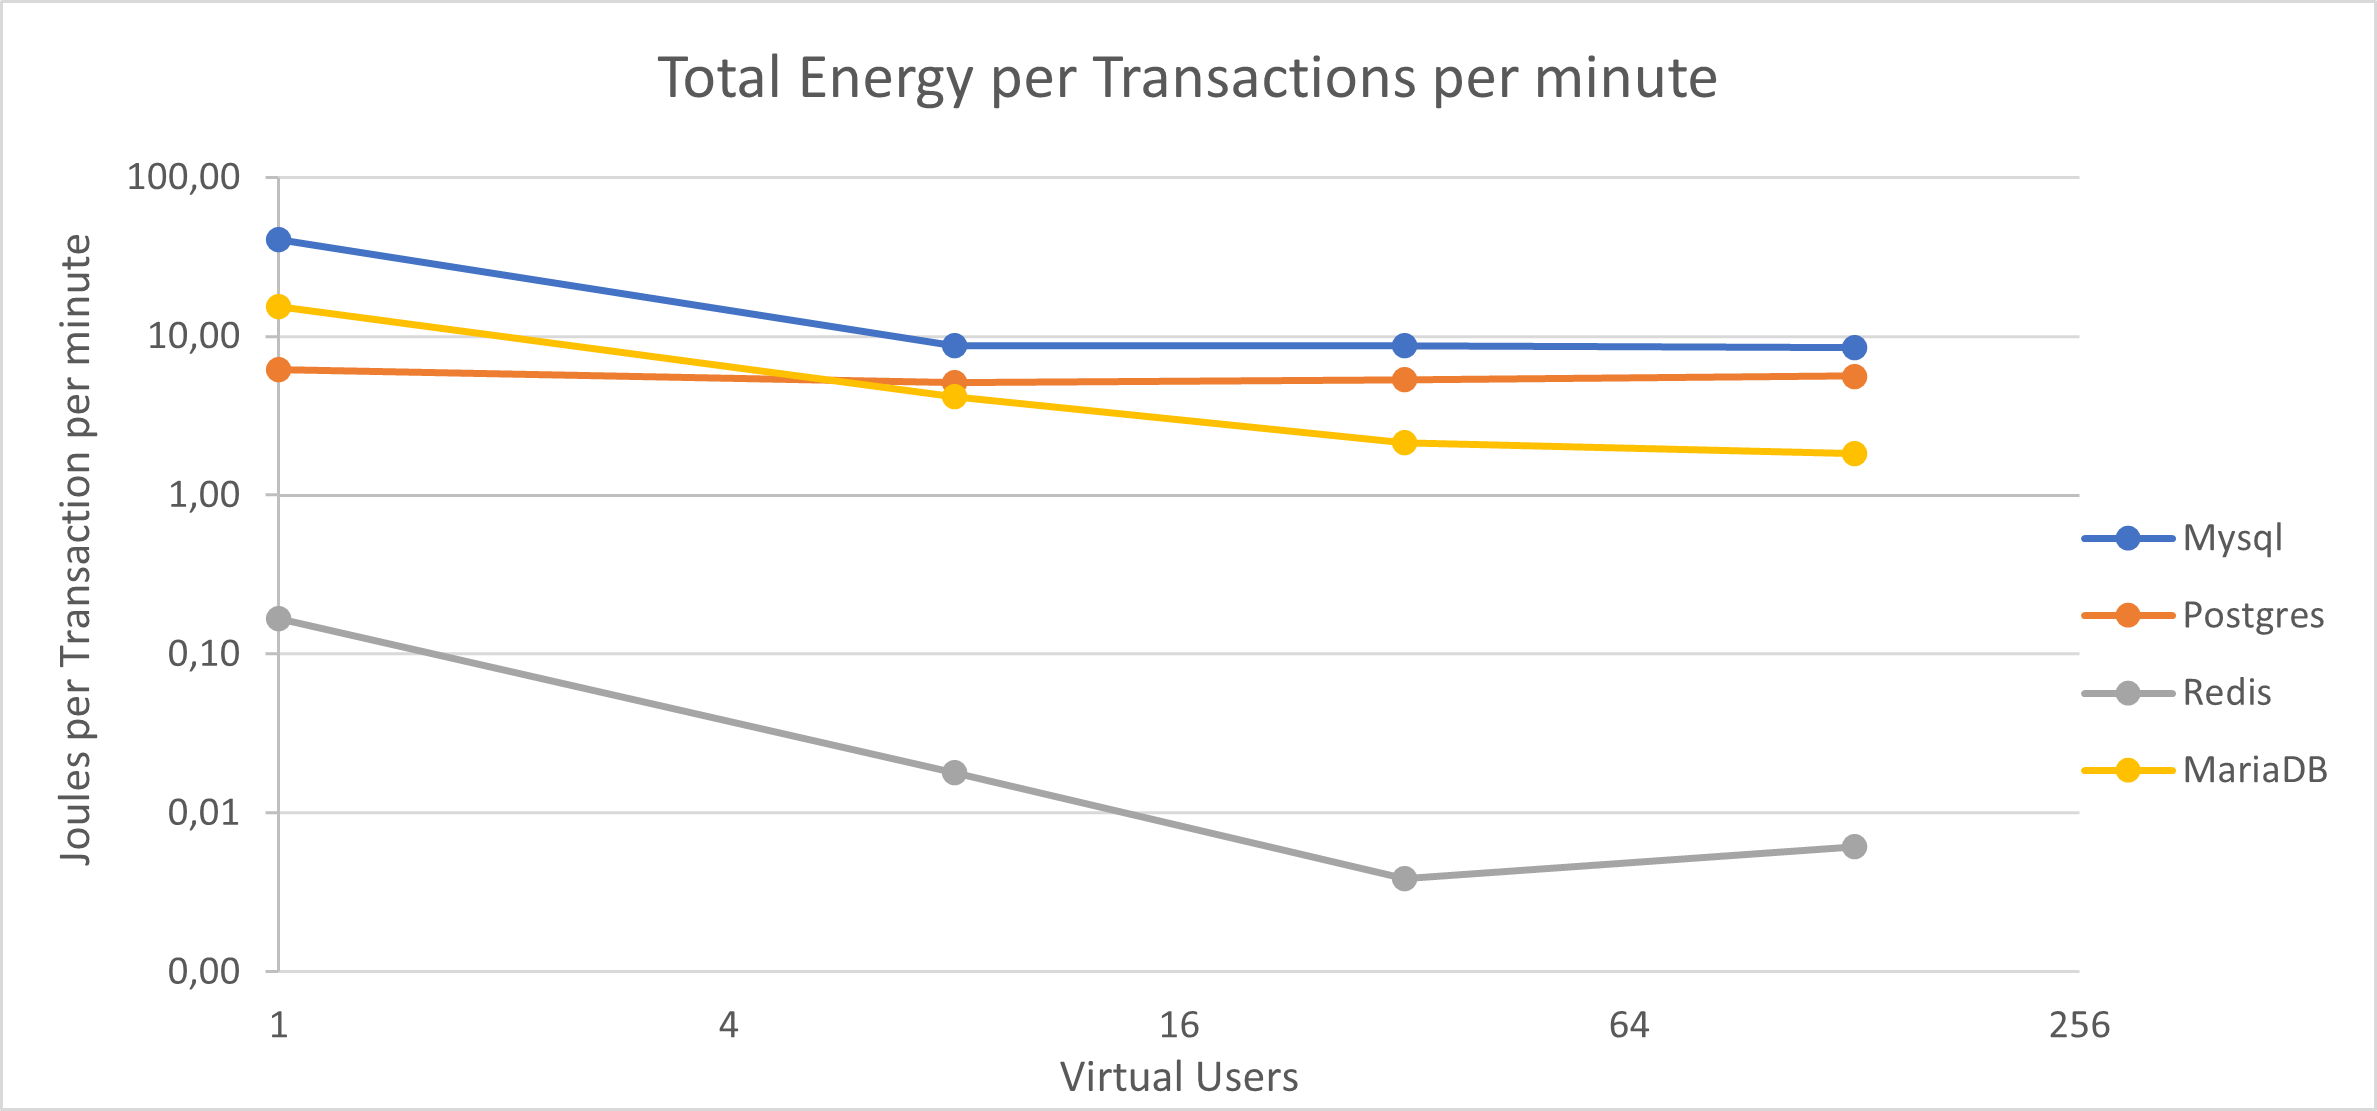
\includegraphics[width=1\columnwidth]{results/vu/total-tpm.png}
            \caption[]%
            {{\small Energy consumption on System per TPM with different number users}}    
            \label{fig:vutranstotal}
        \end{subfigure}
        \caption[ Energy consumption per TPM with different number users ]
        {\small Energy consumption per TPM with different number users} 
        \label{fig:vuyenergytpm}
    \end{figure}
   
    %explicar tudo
    Finally, in Figure \ref{fig:vuyenergynopm} we can check the energy consumption per \gls{nopm}, we can see that all DBMS improve very well and we can see that Redis became the most efficient on energy consumption per 
        %explicar tudo
\gls{nopm} with the increase of users, follow by MariaDB, Postgres, and MySQL. These improvements are very similar to the improvement in energy consumption per \gls{tpm} where the decrease of energy consumption on disk per \gls{nopm} has a great impact on total energy consumption per \gls{nopm}.
    
\begin{figure}[h!]
        \centering
        \begin{subfigure}[b]{0.42\textwidth}
            \centering
			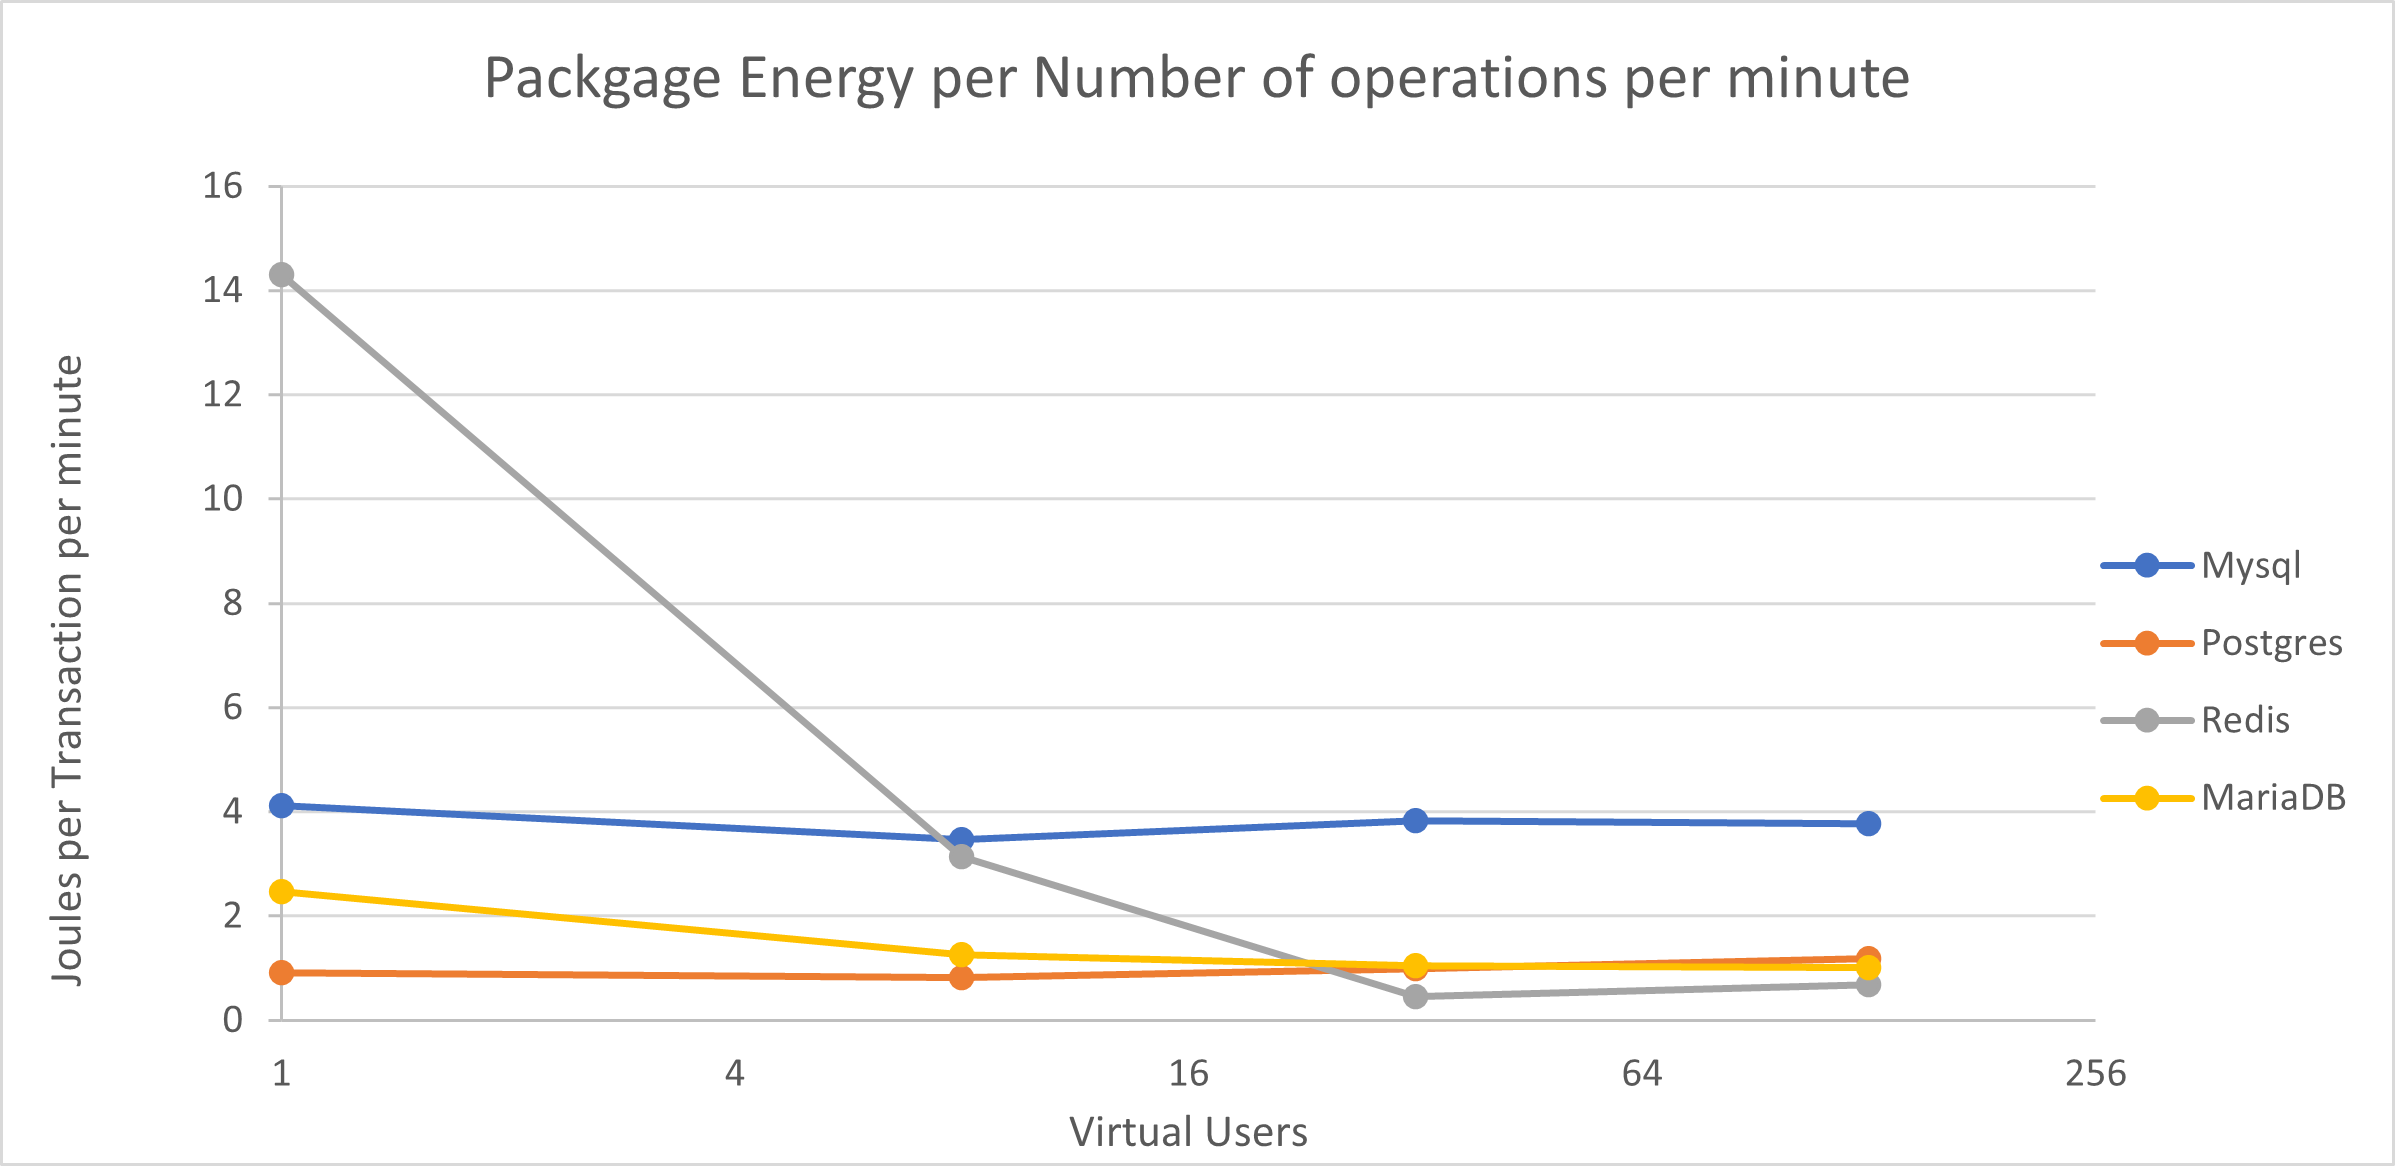
\includegraphics[width=1\columnwidth]{results/vu/Packgage-nopm.png}
			\caption[]%
            {{\small Energy consumption on Package per NOPM with different number of users}}    
			\label{fig:vuyenergynopmpackage}
        \end{subfigure}
        \hfill
        \begin{subfigure}[b]{0.42\textwidth}  
            \centering 
            \includegraphics[width=1\columnwidth]{results/vu/Disk-nopm.png}
            \caption[]%
            {{\small Energy consumption on Disk per NOPM with different number of users}}    
            \label{fig:vuyenergynopmdisk}
        \end{subfigure}
        \vskip\baselineskip
        \begin{subfigure}[b]{0.42\textwidth}  
            \centering 
            \includegraphics[width=1\columnwidth]{results/vu/total-nopm.png}
            \caption[]%
            {{\small Energy consumption on System per NOPM with different number users}}    
            \label{fig:vuyenergynopmtotal}
        \end{subfigure}
        \caption[ Energy consumption per NOPM with different number of users ]
        {\small Energy consumption per NOPM with different number of users} 
        \label{fig:vuyenergynopm}
    \end{figure}
   

  On an overall note, it can be concluded that that the non relational \gls{dbms} Redis start to get better results on  \gls{nopm} and \gls{tpm} without a large increase in energy consumption making Redis the most scalable one. When talking about relational \gls{dbms}, MariaDB had the most increase in HammerDB performance and energy consumption per \gls{tpm} and \gls{nopm} with the increase of users and Postgres maintain or get worse results comparing with only one virtual user.




%\discuss{não tentes repsonder ás perguntas enquanto apresentas os resultados. No fim deste capitulo, ou nas conclusoes, é que as referes e respondes.}







